\documentclass[11pt,a4paper]{article}

\usepackage[utf8]{inputenc}
\usepackage[expansion=false]{microtype}
\usepackage[margin=1in]{geometry}
\usepackage{amsmath,amssymb,amsthm,mathtools}
\usepackage{booktabs}
\usepackage{array}
\usepackage{multirow}
\usepackage{enumitem}
\usepackage{xcolor}
\usepackage{tikz}
\usetikzlibrary{arrows.meta,positioning,calc,shapes.geometric,fit,backgrounds,matrix}
\usepackage{hyperref}

\definecolor{accent}{RGB}{24,90,168}
\definecolor{accentlight}{RGB}{232,241,250}

\hypersetup{
    colorlinks=true,
    linkcolor=black!80,
    citecolor=black!80,
    urlcolor=black!80,
    pdftitle={Algebraic Cryptanalysis of LOCKER and ROLLO},
    pdfauthor={MiniMax}
}

\newtheorem{theorem}{Theorem}
\newtheorem{lemma}[theorem]{Lemma}
\newtheorem{proposition}[theorem]{Proposition}
\newtheorem{corollary}[theorem]{Corollary}
\theoremstyle{definition}
\newtheorem{definition}[theorem]{Definition}
\theoremstyle{remark}
\newtheorem{remark}[theorem]{Remark}

\newcommand{\F}{\mathbb{F}}
\newcommand{\Ftwo}{\mathbb{F}_2}
\newcommand{\GL}{\mathrm{GL}}
\newcommand{\Gr}{\mathrm{Gr}}
\newcommand{\Supp}{\operatorname{Supp}}
\newcommand{\rk}{\operatorname{rank}}
\newcommand{\RREF}{\operatorname{RREF}}
\newcommand{\diag}{\operatorname{diag}}
\newcommand{\lcm}{\operatorname{lcm}}
\newcommand{\TSM}{\mathsf{TSM}}
\newcommand{\RSR}{\mathsf{RSR}}
\newcommand{\SHA}{\mathsf{SHA512}}
\newcommand{\XOF}{\mathsf{XOF}}
\newcommand{\algstep}[2]{\hangindent=2.4em\hangafter=1\hspace*{1.1em}\textbf{#1.} #2}

\title{\bfseries Algebraic Cryptanalysis of LOCKER and ROLLO}
\author{MiniMax}
\date{November 2026}

\begin{document}
\maketitle

\begin{abstract}
Ideal Low-Rank Parity-Check (LRPC) key encapsulation mechanisms replace Hamming weight with rank weight over a binary polynomial quotient ring. They were submitted to the first round of the NIST Post-Quantum Cryptography standardization process as Low-Rank Parity-Check Codes Encryption (LOCKER), Low-Rank Parity-Check Key Exchange (LAKE), and Rank-Ouroboros, and merged in the second round as Rank-Ouroboros, LAKE, and LOCKER (ROLLO). Because an irreducible binary modulus of degree $n$ over $\F_{2^m}$ eliminates proper ideals when $m$ and $n$ are coprime, prior algebraic attacks unfold ring multiplication into a generic linear code of length $2n$ over $\F_{2^m}$, requiring hundreds of millions of minor variables and petabytes of memory on first-round parameters.

In this paper, we show that the irreducibility of the ring modulus enables a direct algebraic attack whenever the field extension degree $m$ exceeds $2^r$ for error rank $r$ or $2^d$ for secret key rank $d$. Because the binary quotient ring modulo the irreducible polynomial is itself the extension field $\F_{2^n}$, transposing the $n \times m$ binary coefficient matrix maps the scheme ring isomorphically onto a polynomial quotient ring over $\F_{2^n}$. Under this transposition, any subspace of the original base field $\F_{2^m}$ consists of polynomials with binary coefficients and is fixed pointwise by squaring coefficients in $\F_{2^n}$. Iterating this partial Frobenius automorphism generates an orbit of conjugate equations over the identical unknown support from a single passive ciphertext or public key with zero decapsulation queries. We derive polynomial-time ciphertext support recovery via local Schur elimination when $m > 2^r$, and direct public-key secret recovery via principal minors and a closed-form Moore-matrix gauge recursion when $m \ge 2^d$. Across all $27$ published parameter sets ($24$ official NIST submission sets from 2017--2020 and $3$ additional new2ROLLO-I sets), our attacks improve upon the best published complexities on $14$ sets---recovering the shared secret of LOCKER-I in $1.15\text{ s}$ using $58\text{ MB}$ of memory on a $12$-thread workstation and recovering the $2019$ ROLLO-I-128 secret key in $5.97\text{ s}$ on a single core---while proving via exact Frobenius syzygy counts that the $2020$ revised ROLLO and new2ROLLO-I parameter sets with $m \le 2^r$ and $m < 2^d$ remain immune.
\end{abstract}

\section{Introduction}
\label{sec:intro}

\subsection{Background and Design Rationale}
Code-based public-key cryptosystems in the Hamming metric, such as Classic McEliece, require public keys of several hundred kilobytes because information-set decoding scales only linearly with the error weight in the exponent. Rank-metric cryptography replaces Hamming weight over $\Ftwo$ with the $\Ftwo$-rank of vectors over an extension field $K \cong \F_{2^m}$. Because generic Rank Syndrome Decoding ($\mathsf{RSD}$) algorithms scale quadratically with $m$ and the rank weight $r$ in the exponent, rank-metric constructions achieve $128$-bit security with public keys under one kilobyte.

Introduced by Gaborit, Murat, Ruatta, and Z\'{e}mor~\cite{GMRZ13}, Ideal Low-Rank Parity-Check ($\mathsf{LRPC}$) cryptosystems compress keys to a single ring element by operating in the polynomial quotient ring $R = K[X]/(P(X))$ of degree $n$. A secret key consists of a $d$-dimensional $\Ftwo$-subspace $F \subset K$ and two polynomials $x, y \in F^n$ whose coefficients lie in $F$, while the public key is the quotient $h = x^{-1} y \bmod P(X)$ ($747$~bytes in $\mathsf{LOCKER\text{-}I}$). Encapsulation samples an $r$-dimensional $\Ftwo$-subspace $E \subset K$ and error polynomials $e_1, e_2 \in E^n$, outputting the syndrome $u = e_1 + e_2 h \bmod P(X)$. Decapsulation computes $s = x u \equiv x e_1 + y e_2 \pmod{P(X)}$, whose coefficients lie in the product subspace $F \cdot E$ of dimension at most $r d < m$, and intersects $f_i^{-1}\Supp(s)$ across a basis of $F$ to recover $E$.

Across the NIST Post-Quantum Cryptography standardization process and contemporaneous cryptanalytic literature, $27$ Ideal-LRPC parameter sets ($24$ official submission sets and $3$ literature sets) were specified across four parameter families. In November 2017 (NIST Round~1), Aragon et al.~\cite{LOCKER17} submitted three sister schemes: $\mathsf{LAKE}$ (an ephemeral IND-CPA KEM), $\mathsf{LOCKER}$ (an IND-CCA2 KEM with nine parameter sets $\mathsf{LOCKER\text{-}I..IX}$ at $r \in \{5, 6\}$ and $d \in \{7, 8, 9\}$ designed for decryption failure rates below $2^{-64}$), and $\mathsf{Rank\text{-}Ouroboros}$. In March 2019 (NIST Round~2~\cite{ROLLO19}), the three submissions were merged into $\mathsf{ROLLO\text{-}I}$ ($\mathsf{LAKE}$), $\mathsf{ROLLO\text{-}II}$ ($\mathsf{LOCKER}$), and $\mathsf{ROLLO\text{-}III}$ ($\mathsf{Rank\text{-}Ouroboros}$), comprising nine parameter sets with $r \in \{5, 6, 7\}, d \in \{6, 7, 8\}$ on $\mathsf{ROLLO\text{-}I/II}$ and secret-key rank $d = w \in \{5, 6, 7\}$, error rank $r = w_r \in \{6, 8, 8\}$ on $\mathsf{ROLLO\text{-}III}$. Following the algebraic attacks of Bardet et al.~\cite{BBB+20,BBC+20}---where~\cite{BBC+20} also proposed three illustrative large-$m$ parameter sets $\mathsf{new2ROLLO\text{-}I\text{-}128/192/256}$ ($m \in \{73, 89, 103\}$, $r \in \{7, 8, 9\}$, later re-evaluated in~\cite{BBGT23})---the April 2020 Round~2 revision~\cite{ROLLO20} dropped $\mathsf{ROLLO\text{-}III}$ and raised $(r, d)$ to $7\text{--}9$ across six sets ($\mathsf{ROLLO\text{-}I/II\text{-}128/192/256}$). In July 2020, NIST declined to advance $\mathsf{ROLLO}$ to Round~3~\cite{NISTIR8309}, citing rapid progress in algebraic cryptanalysis of rank-metric codes.

\subsection{Prior Cryptanalysis}
Prior cryptanalysis of Ideal-LRPC schemes follows four main directions, summarized in Table~\ref{tab:intro-sota}. First, Hauteville and Tillich~\cite{HT15} showed that when $P(X)$ factors over $\Ftwo$ (as in quasi-cyclic rings modulo $X^n - 1$), projecting modulo a proper factor shortens the code length while preserving the rank bound $r$. To block quotient-ring folding, all $27$ published $\mathsf{LOCKER}$ and $\mathsf{ROLLO}$ parameter sets choose an irreducible binary polynomial $P(X) \in \Ftwo[X]$ with $\gcd(m, n) = 1$, so that $R \cong \F_{2^{mn}}$ is an extension field with no proper ideals. Chee et al.~\cite{CJL+24} separately analyzed a modified layered $\mathsf{ROLLO\text{-}I}$ variant with restricted error degrees $\deg(e_i) \ll n$, which does not apply to standard full-degree errors.

Second, combinatorial subspace-guessing attacks~\cite{GMRZ13,LOCKER17} cost $\widetilde{O}(2^{(r-1)\lceil m(n+1)/(2n)\rceil})$ operations ($2^{144}$ on $\mathsf{LOCKER\text{-}I}$). Decryption-failure reaction attacks~\cite{SSL19} require approximately $\mathrm{DFR}^{-1} \ge 2^{64}$ active decapsulation queries on $\mathsf{LOCKER}$ and do not apply to ephemeral $\mathsf{ROLLO\text{-}I}$. Third, the structural dual-LRPC key recovery attack analyzed in the $\mathsf{ROLLO}$ specification~\cite[\S6.2]{ROLLO20} and evaluated across the $2020$ parameters by Song et al.~\cite{SZHW23} searches for rank-$d$ multiples of $(y, -x)$ up to $n$ ring shifts in $O((nm)^\omega 2^{d\lceil m/2\rceil - m - n})$ operations. This structural attack requires $2^{133}$ operations on $\mathsf{LOCKER\text{-}I}$ and reduces four $2020$ sets below their claimed security ($2^{103.2}\text{--}2^{180.3}$), whereas $2020$ $\mathsf{ROLLO\text{-}I\text{-}128/256}$ and all $\mathsf{new2ROLLO\text{-}I}$ sets remain above claimed levels.

\begin{table}[t]
\centering
\caption{Comparison of passive attacks ($0$ decapsulation queries) on $\mathsf{LOCKER\text{-}I}$ and $2019$ $\mathsf{ROLLO\text{-}I\text{-}128}$. Column counts give the number of linearized minor variables after optimal puncturing or Schur reduction; complexities are reported in $\log_2$ two-input gates.}
\label{tab:intro-sota}
\setlength{\tabcolsep}{5.0pt}
\begin{tabular}{@{}llcccc@{}}
\toprule
\textbf{Reference} & \textbf{Attack Method} & \textbf{Columns} & \textbf{Memory} & \textbf{Gates} & \textbf{Time} \\
\midrule
\multicolumn{6}{@{}l}{\emph{Target: $\mathsf{LOCKER\text{-}I}$ $(m=71, n=83, r=5, d=7$; claimed $128$-bit IND-CCA2)}} \\
Aragon et al.~\cite{LOCKER17} & Combinatorial RSD & --- & --- & $2^{144.0}$ & --- \\
Hauteville--Tillich~\cite{HT15} & Quotient folding & --- & --- & N/A & --- \\
Bardet et al.~\cite{BBC+20} & MaxMinors ($\omega = 2.81$) & $5.72 \times 10^8$ & $42\text{ PB}$ & $2^{81.8}$ & --- \\
Esser et al.~\cite{EVV26} & MaxMinors ($\omega = 2$) & $5.72 \times 10^8$ & $42\text{ PB}$ & $2^{58.2}$ & --- \\
This Work (Sec.~\ref{subsec:ct-schur}) & Schur $\TSM$ ($P = 9$) & $2{,}240$ & $58\text{ MB}$ & $2^{45.6^\dagger}$ & $1.15\text{ s}$ \\
This Work (Sec.~\ref{subsec:ct-sparse}) & Sparse Lanczos $\TSM$ & $4{,}032$ & $18\text{ MB}$ & $2^{46.3}$ & --- \\
\midrule
\multicolumn{6}{@{}l}{\emph{Target: $2019$ $\mathsf{ROLLO\text{-}I\text{-}128}$ $(m=79, n=47, r=5, d=6$; claimed $128$-bit IND-CPA)}} \\
Bardet et al.~\cite{BBC+20} & MaxMinors ($\omega = 2.81$) & $3.28 \times 10^7$ & $141\text{ TB}$ & $2^{70.2}$ & --- \\
Esser et al.~\cite{EVV26} & MaxMinors ($\omega = 2$) & $3.28 \times 10^7$ & $141\text{ TB}$ & $2^{50.0}$ & --- \\
This Work (Sec.~\ref{subsec:ct-schur}) & Schur $\TSM$ ($P = 8$) & $1{,}120$ & $48\text{ MB}$ & $2^{42.2}$ & --- \\
This Work (Sec.~\ref{subsec:pk-closed}) & Direct key recovery & $64$ & $< 2\text{ MB}$ & $2^{31.3}$ & $5.97\text{ s}$ \\
\bottomrule
\end{tabular}
\\[0.3em]
{\scriptsize $^\dagger$Evaluated in the $2n^2$ two-input gate model on the $2184 \times 2240$ Schur-reduced matrix over $\F_{2^{83}}$ ($2^{39.7}$ under the $n = \log_2 q$ field-operation metric of~\cite{EVV26}).}
\end{table}

Fourth, the algebraic MaxMinors and Support-Minors attacks introduced by Bardet et al.~\cite{BBB+20,BBC+20,BBGT23} and further analyzed by Couv\'{e}e et al.~\cite{CWZ26} and Esser, Verbel, and Villanueva-Polanco~\cite{EVV26} expand multiplication modulo $P(X)$ into an $n \times n$ companion matrix over $K = \F_{2^m}$ and treat $(e_1, e_2)$ as a generic $[2n, n]$ linear code over $K$. Even after optimal puncturing ($p = 17$ on $\mathsf{LOCKER\text{-}I}$ and $p = 9$ on $2019$ $\mathsf{ROLLO\text{-}I\text{-}128}$), linearizing $(r+1)\times(r+1)$ maximal minors requires $\binom{2n - p}{r} = \binom{149}{5} = 5.72 \times 10^8$ columns ($\approx 42\text{ PB}$ dense memory) on $\mathsf{LOCKER\text{-}I}$ and $\binom{85}{5} = 3.28 \times 10^7$ columns ($\approx 141\text{ TB}$ dense memory) on $2019$ $\mathsf{ROLLO\text{-}I\text{-}128}$. In the standard ring representation $R = K[X]/(P(X))$, one cannot generate extra equations over the same support $E = \langle b_1, \dots, b_r \rangle_{\Ftwo} \subset K$ by squaring $K$-coefficients, because the Frobenius map on $K$ sends
\[
    e_i(X) = \sum_{k=1}^{r} b_k\, a_{i,k}(X) \;\longmapsto\; \sum_{k=1}^{r} b_k^2\, a_{i,k}(X) \qquad (a_{i,k}(X) \in \Ftwo[X]/(P(X))),
\]
which shifts $E$ to a distinct subspace $E^{[1]} = \langle b_1^2, \dots, b_r^2 \rangle_{\Ftwo} \neq E$. For this reason, the $\mathsf{ROLLO}$ specifications and subsequent rank-metric security analyses~\cite{ROLLO20,AAD+22,ABD+24} concluded that choosing an irreducible modulus $P(X)$ prevents ideal structure from accelerating syndrome decoding.

\subsection{Our Contributions}
We show that the irreducibility of $P(X) \in \Ftwo[X]$---introduced specifically to defeat quotient-ring folding~\cite{HT15}---makes the binary quotient ring $L = \Ftwo[X]/(P(X)) \cong \F_{2^n}$ a field and unlocks a partial Frobenius action that preserves the secret support. Transposing the $n \times m$ binary coefficient matrix exchanges the roles of $X$ and $T$, mapping $R = K[X]/(P(X))$ isomorphically onto $Q = L[T]/(g(T))$. In $Q$, each binary polynomial $a_{i,k}(X)$ becomes a field scalar in $L$, whereas each support basis element $b_k(T) \in K$ becomes a polynomial in $T$ with $\{0, 1\}$ coefficients, fixed pointwise by squaring $L$-coefficients via $\rho(\sum_t \gamma_t T^t) = \sum_t \gamma_t^2 T^t$. Iterating $\rho$ on a single passive ciphertext or public key generates up to $n$ conjugate equations over the identical support basis:

\begin{enumerate}[leftmargin=1.8em,itemsep=2pt]
    \item \textbf{Transposed Partial Frobenius Orbit (Section~\ref{sec:transpose}, Lemma~\ref{lem:transpose}):} Building on the classical transposition duality of matrix codes~\cite{Delsarte78}, we prove that $\Phi: R \xrightarrow{\sim} Q = L[T]/(g(T))$ identifies $\Phi(K) = \Ftwo[T]/(g(T))$ with the fixed subring $Q^\rho$, satisfies $(L \otimes_{\Ftwo} E) \cap \Phi(K) = \Phi(E)$, and generates an orbit of conjugate syndrome equations $U_q = \rho^q(U_0)$ over the unchanged support $\Phi(E)$.
    \item \textbf{Ciphertext Support Recovery for $m > 2^r$ (Section~\ref{sec:ct-attacks}, Lemma~\ref{lem:row-complete}, Propositions~\ref{prop:schur}--\ref{prop:split-ring}, Theorem~\ref{thm:ct-threshold}):} Adapting the Support-Minors cofactor expansion of Bardet et al.~\cite{BBC+20,BBGT23} to the commutative ring $Q$ across $P \ll n$ Frobenius conjugates restricts the minor unknowns to $\binom{P}{r}2^r$ pair-transversal minors in $L$, where each non-pivot subset $0 \notin S_i$ forms a local $m \times 2^r$ block $B_i$. When $m > 2^r$ and $P \ge P_2^*(m, r) = \lceil(mr - 2^r)/(m - 2^r)\rceil \le n$, local Schur elimination collapses $\mathsf{LOCKER\text{-}I}$ from $5.72 \times 10^8$ columns ($42\text{ PB}$) to $2{,}240$ columns ($58\text{ MB}$), recovering the shared secret in $1.15\text{ s}$ on a $12$-thread CPU. For $r = 6$, retaining the unreduced block-staircase matrix yields constant row weight $w = (r+1)2^r = 448$, compressing $\mathsf{LOCKER\text{-}III/VI/IX}$ from $565\text{--}863\text{ GB}$ dense storage into $1.65\text{--}2.35\text{ GB}$ compressed sparse row ($\mathsf{CSR}$) format ($2^{58.8}\text{--}2^{60.5}$ gates). We also prove that $X^n - 1$ quotients and non-coprime degrees $\gcd(m, n) > 1$ remain vulnerable via cyclotomic projection.
    \item \textbf{Direct Public-Key Recovery for $m \ge 2^d$ (Section~\ref{sec:pk-attacks}, Theorems~\ref{thm:pk-minors}--\ref{thm:moore-rec}, Proposition~\ref{prop:window}):} We prove that when $m \ge 2^d$, the $m \times 2^d$ matrix $C_H$ formed by subset products of $H_0, \dots, H_{d-1}$ has a one-dimensional $L$-kernel whose entries equal all $2^d$ principal minors of the Moore transition matrix $M = B A^{-1} \in \GL_d(L)$. Whereas classical principal-minor reconstruction~\cite{Loewy86,GT06} determines $\tilde{M}$ only up to an unknown diagonal similarity $M = D \tilde{M} D^{-1}$ in $(L^\times)^{d-1}$ and transposition, we derive a closed-form Moore-row recursion for $D$ from the uniqueness of the subspace annihilator polynomial $\mathcal{L}_\alpha(Z)$. On homogeneous Ideal-LRPC public keys $h = x^{-1} y \bmod P(X)$, this recovers the secret key $(F, x, y)$ from $h$ alone in $5.97\text{ s}$ on $2019$ $\mathsf{ROLLO\text{-}I\text{-}128}$ on a single core (whereas inhomogeneous $2019$ $\mathsf{ROLLO\text{-}III\text{-}128/192}$ public keys $\mathsf{pk} = (h, s = x + h y)$ are solved directly by Section~\ref{sec:ct-attacks} in $2^{39.3}$ and $2^{57.6}$ gates).
    \item \textbf{Phase Transitions and $27$-Set Security Ledger (Sections~\ref{sec:barriers}--\ref{sec:evaluation}, Theorem~\ref{thm:dichotomy}):} We prove that in the sub-threshold regime $m \le 2^r$, the exact $\Ftwo$-nullity is $\nu_{\Ftwo}(P) = n[2^r\binom{P-1}{r-1} - m\binom{P-2}{r-1}]$, which grows strictly with $P$ and leaves quadratic Grassmannian Pl\"{u}cker relations underdetermined by factors of $6.5 \times 10^3$ to $1.07 \times 10^5$. Evaluating all $27$ published parameter sets shows that our attacks improve upon published 2026 complexities on $14$ sets (all $9$ Round~1 $\mathsf{LOCKER}$ sets and $5$ of $9$ initial Round~2 $\mathsf{ROLLO}$ sets), while all $6$ revised Round~2 $\mathsf{ROLLO}$ sets (2020) and all $3$ $\mathsf{new2ROLLO\text{-}I}$ sets~\cite{BBC+20} satisfy $m < 2^r, 2^d$ and remain immune.
\end{enumerate}

\subsection{Paper Organization}
Section~\ref{sec:prelim} establishes our algebraic notation and reviews rank syndrome decoding, Ideal-LRPC codes, Support-Minors linearization, Moore matrices, and the Principal Minor Assignment Problem. Section~\ref{sec:spec} gives the formal specification of $\mathsf{LOCKER}$ and $\mathsf{ROLLO}$ across all four parameter generations. Section~\ref{sec:transpose} introduces the transposed ring isomorphism $\Phi$ and proves support invariance under the partial Frobenius $\rho$. Section~\ref{sec:ct-attacks} develops our ciphertext support-recovery attacks. Section~\ref{sec:pk-attacks} presents our direct public-key recovery attack and transposed subspace search. Section~\ref{sec:barriers} proves the exact nullity formula and quadratic Pl\"{u}cker barriers for $m \le 2^r$. Section~\ref{sec:evaluation} presents the complete $27$-set complexity ledger and experimental verification benchmarks.

\section{Preliminaries}
\label{sec:prelim}

\subsection{Finite Fields and Quotient Rings}
Let $\Ftwo = \{0, 1\}$ denote the binary field. Given an irreducible binary polynomial $g(T) \in \Ftwo[T]$ of degree $m$, we denote by $K \coloneqq \Ftwo[T]/(g(T)) \cong \F_{2^m}$ the degree-$m$ extension field viewed as an $m$-dimensional vector space over $\Ftwo$ with power basis $(1, T, \dots, T^{m-1})$. Let $P(X) \in \Ftwo[X]$ be a monic binary polynomial of degree $n$. The polynomial quotient ring over $K$ is
\[
    R \coloneqq K[X] / (P(X)) = \left\{ \sum_{j=0}^{n-1} a_j X^j : a_j \in K \right\}.
\]
Expanding each coefficient $a_j = \sum_{t=0}^{m-1} \mu_{j,t} T^t \in K$ ($\mu_{j,t} \in \Ftwo$) associates to every ring element $a \in R$ a unique binary coefficient matrix $M(a) \coloneqq (\mu_{j,t})_{0 \le j < n,\, 0 \le t < m} \in \Ftwo^{n \times m}$.

The \emph{rank support} of $a \in R$, denoted $\Supp(a) \coloneqq \langle a_0, \dots, a_{n-1} \rangle_{\Ftwo} \subseteq K$, is the $\Ftwo$-subspace of $K$ spanned by the coefficients of $a(X)$. Its dimension $\rk_{\Ftwo}(a) \coloneqq \dim_{\Ftwo}\Supp(a) = \rk_{\Ftwo} M(a)$ is the rank weight of $a$. An element $e \in R$ satisfies $\Supp(e) \subseteq E$ for an $r$-dimensional subspace $E = \langle b_1, \dots, b_r \rangle_{\Ftwo} \subset K$ if and only if $\rk_{\Ftwo} M(e) \le r$, or equivalently if $e(X)$ admits the rank-$r$ decomposition
\begin{equation}
\label{eq:rank-decomp}
    e(X) = \sum_{k=1}^{r} b_k \, a_k(X), \qquad b_k \in K,\quad a_k(X) \in \Ftwo[X]/(P(X)).
\end{equation}
In matrix terms,~\eqref{eq:rank-decomp} expresses $M(e) \in \Ftwo^{n \times m}$ as a sum of $r$ outer products of column vectors in $\Ftwo^n$ and row vectors in $\Ftwo^m$. By Delsarte's classical duality for matrix codes~\cite{Delsarte78}, transposing $M(e) \mapsto M(e)^\top \in \Ftwo^{m \times n}$ preserves the $\Ftwo$-rank $r$ while exchanging the roles of the column space over $\Ftwo^n$ and the row space over $\Ftwo^m$.

We denote by $\Gr_{\Ftwo}(r, K)$ the Grassmannian of all $r$-dimensional $\Ftwo$-subspaces of $K$, whose cardinality is given by the Gaussian binomial coefficient
\[
    \bigl|\Gr_{\Ftwo}(r, K)\bigr| = \genfrac{[}{]}{0pt}{}{m}{r}_2 \coloneqq \prod_{i=0}^{r-1} \frac{2^m - 2^i}{2^r - 2^i}.
\]
For any $r$-dimensional subspace $E \subset K$, we write $\RREF(E) \in K^r$ for the canonical basis of $E$ whose $r \times m$ binary matrix in the basis $(1, T, \dots, T^{m-1})$ is in reduced row-echelon form.

\subsection{Rank Syndrome Decoding and Ideal-LRPC Codes}
The security of $\mathsf{LOCKER}$ and $\mathsf{ROLLO}$ rests on the Rank Syndrome Decoding ($\mathsf{RSD}$) problem and its ring-structured specialization to Ideal-LRPC codes~\cite{GMRZ13,LOCKER17,ROLLO20}.

\begin{definition}[Ideal Rank Syndrome Decoding and Low-Rank Parity-Check Codes~\cite{GMRZ13,ROLLO20}]
\label{def:ideal-rsd}
Let $R = K[X]/(P(X))$ with $K = \F_{2^m}$ and $\deg P = n$. In the Ideal-$\mathsf{RSD}(m, n, r)$ distribution, a public polynomial $h \in R$ is given alongside a syndrome $u = e_1 + e_2 h \bmod P(X)$, where $E \xleftarrow{\$} \Gr_{\Ftwo}(r, K)$ is a uniform $r$-dimensional support and $e_1, e_2 \xleftarrow{\$} E^n$ are sampled uniformly among polynomials of full support $\Supp(e_1) = \Supp(e_2) = E$. An Ideal-$\mathsf{LRPC}(m, n, d)$ public key replaces uniform $h \in R$ with $h = x^{-1} y \bmod P(X)$, where $F \xleftarrow{\$} \Gr_{\Ftwo}(d, K)$ is a secret $d$-dimensional support and $x, y \xleftarrow{\$} F^n$ with $x \in R^\times$.
\end{definition}

For any two $\Ftwo$-subspaces $F, E \subset K$ of dimensions $d$ and $r$, their product subspace $F \cdot E \coloneqq \langle f e : f \in F,\, e \in E \rangle_{\Ftwo} \subseteq K$ has dimension at most $r d$. When $r d < m$, multiplying the syndrome $u = e_1 + e_2 h$ by the secret polynomial $x \in F^n$ yields $s = x u \equiv x e_1 + y e_2 \pmod{P(X)}$ whose coefficients lie entirely in $F \cdot E$, enabling decoding by subspace intersection~\cite{GMRZ13}.

\subsection{Support-Minors Modeling and Moore Matrices}
Our cryptanalysis builds upon and extends three algebraic tools from rank-metric cryptanalysis and linear algebra:

\paragraph{Support-Minors and MaxMinors Linearization~\cite{BBC+20,BBGT23}.}
In a generic $[N, k]$ linear code over $K = \F_{2^m}$ with parity-check matrix $H_{\text{pub}} \in K^{(N-k) \times N}$, a rank-$r$ error vector $e = C b^\top \in K^N$ factors through a basis $b \in K^r$ of $E$ and a binary coordinate matrix $C \in \Ftwo^{N \times r}$ of rank $r$. Bardet et al.~\cite{BBC+20,BBGT23} observed that for any syndrome equation, augmenting $C^\top$ with a syndrome-combination row produces an $(r+1) \times N$ matrix of rank $r$ whose $(r+1) \times (r+1)$ maximal minors vanish. Expanding these determinants along the augmented row expresses every equation as a linear combination of the $\binom{N}{r}$ maximal minors (Pl\"{u}cker coordinates) of $C$. When applied directly to an Ideal-LRPC instance over $R = K[X]/(P(X))$ of length $N = 2n$, this modeling requires $\binom{2n-p}{r}$ minor columns after puncturing $p$ positions.

\paragraph{Moore Matrices and Subspace Annihilator Polynomials.}
For elements $\alpha_1, \dots, \alpha_d$ in a characteristic-$2$ field $L$, the $d \times d$ Moore matrix is defined by $A \coloneqq (\alpha_k^{2^i})_{0 \le i < d,\, 1 \le k \le d}$. By Moore's determinant theorem, $\det(A) \neq 0$ if and only if $\alpha_1, \dots, \alpha_d$ are linearly independent over $\Ftwo$. In that case, the $d$-dimensional $\Ftwo$-subspace $V_\alpha = \langle \alpha_1, \dots, \alpha_d \rangle_{\Ftwo} \subset L$ is the root set of a unique monic $2$-linearized annihilator polynomial of degree $2^d$:
\[
    \mathcal{L}_\alpha(Z) \coloneqq \prod_{v \in V_\alpha} (Z + v) = Z^{2^d} + \sum_{j=0}^{d-1} c_j Z^{2^j} \in L[Z].
\]

\paragraph{Principal Minor Assignment Problem~\cite{Loewy86,GT06}.}
Given a matrix $M \in L^{d \times d}$ and a subset $Z \subseteq \{0, \dots, d-1\}$, the principal minor $\Delta_Z(M) \coloneqq \det M[Z, Z]$ is the determinant of the $|Z| \times |Z|$ submatrix on row and column indices $Z$ (with $\Delta_\emptyset(M) = 1$). Because $\det(D \tilde{M} D^{-1})[Z, Z] = \det \tilde{M}[Z, Z] = \det \tilde{M}^\top[Z, Z]$ for any invertible diagonal matrix $D = \diag(D_0, \dots, D_{d-1}) \in (L^\times)^d$, the $2^d$ principal minors of $M$ are invariant under both diagonal conjugation and transposition. Conversely, classical results on the Principal Minor Assignment Problem (PMAP) by Loewy~\cite{Loewy86} and Griffin and Tsatsomeros~\cite{GT06} establish that for a generic matrix $M$ with nonzero off-diagonal entries, its principal minors of orders $1, 2,$ and $3$ uniquely determine $M$ up to diagonal conjugation $D$ and transposition $\tilde{M} \leftrightarrow \tilde{M}^\top$. In general, the $(d-1)$-dimensional diagonal gauge $D$ cannot be recovered from the principal minors of $M$ alone; in Section~\ref{subsec:pk-closed}, we show that when $M = B A^{-1}$ links two Moore matrices $A$ and $B$, the Frobenius shift structure of $A$ and $B$ uniquely determines $D$ in closed form.

\section{Specification of LOCKER and ROLLO}
\label{sec:spec}

\subsection{Key Generation, Encapsulation, and Decapsulation}
Table~\ref{tab:scheme-lineage} summarizes the three Ideal-LRPC KEM constructions over $R = K[X]/(P(X))$, Figure~\ref{fig:scheme-arch} illustrates their algebraic workflow, and Algorithms~1 and~2 specify their complete procedures~\cite{LOCKER17,ROLLO19,ROLLO20}.

\begin{table}[t]
\centering
\small
\caption{Summary of the three Ideal-LRPC KEM constructions over $R = \F_{2^m}[X]/(P(X))$ with hash function $H = \SHA$. Here $x, y \in F^n$ have secret support $\dim_{\Ftwo} F = d$, and $e_1, e_2 \in E^n$ have ephemeral error support $\dim_{\Ftwo} E = r$.}
\label{tab:scheme-lineage}
\setlength{\tabcolsep}{4.0pt}
\begin{tabular}{@{}llllc@{}}
\toprule
\textbf{Scheme (R1 / R2)} & \textbf{Goal} & \textbf{$\mathsf{pk}$} & \textbf{Ciphertext $\mathsf{ct}$ and Shared Secret $ss$} & \textbf{$\log_2\mathrm{DFR}$} \\
\midrule
$\mathsf{LAKE}$ / $\mathsf{ROLLO\text{-}I}$ & CPA & $x^{-1}y$ & $e_1 + e_2 h$;\; $ss = H(\RREF(E))$ & $-28\text{..}{-36}$ \\
$\mathsf{LOCKER}$ / $\mathsf{ROLLO\text{-}II}$ & CCA2 & $x^{-1}y$ & $(u, v, d_{\text{tag}})$;\; $ss = H(\mu \parallel u \parallel v)$ & $-64\text{..}{-128}$ \\
$\mathsf{Ouroboros}$ / $\mathsf{ROLLO\text{-}III}$ & CPA & $(h, s_{\text{pk}})^{\mathrm{a}}$ & $(r_0{+}r_1 h,\, e_0{+}r_1 s_{\text{pk}})$;\; $ss = H(\RREF(E))$ & $-28\text{..}{-39}$ \\
\bottomrule
\end{tabular}
\\[0.3em]
{\scriptsize $^{\mathrm{a}}$In $\mathsf{ROLLO\text{-}III}$, $h \xleftarrow{\$} R$ is expanded uniformly from a public seed, $s_{\text{pk}} = w_0 + w_1 h \bmod P(X)$ has secret-key support $\dim_{\Ftwo}\Supp(w_0,w_1) = d = w \in \{5,6,7\}$ ($1 \in \Supp(w_0,w_1)$), and $r_0, r_1, e_0 \in E^n$ share the rank-$r$ error support $E$ with $r = w_r \in \{6,8,8\}$.}
\end{table}

\begin{figure}[t]
\centering
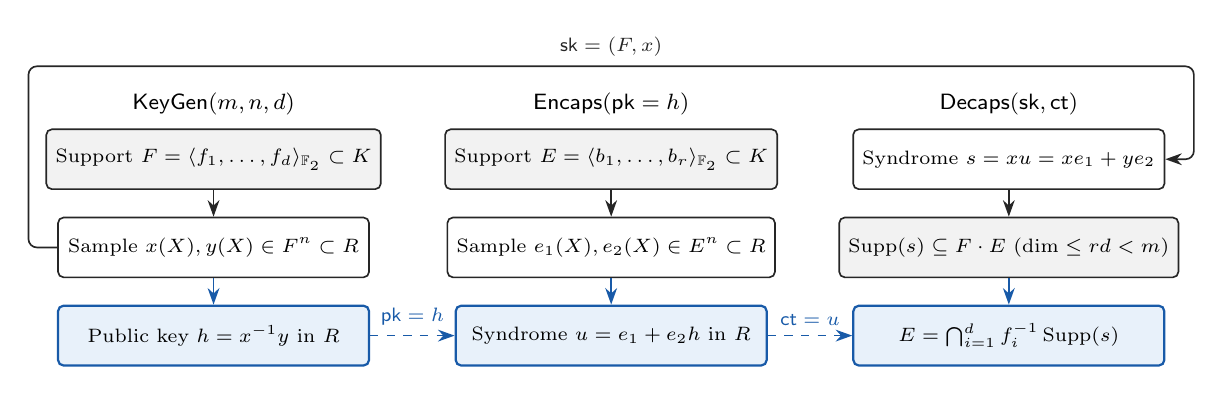
\begin{tikzpicture}[
    font=\scriptsize,
    stagebox/.style={draw=black!85, fill=gray!10, rounded corners=2pt, semithick, minimum width=3.95cm, minimum height=0.76cm, align=center},
    whitebox/.style={draw=black!85, fill=white, rounded corners=2pt, semithick, minimum width=3.95cm, minimum height=0.76cm, align=center},
    accbox/.style={draw=accent, fill=accentlight, rounded corners=2pt, thick, minimum width=3.95cm, minimum height=0.76cm, align=center},
    arr/.style={-{Stealth[length=2.1mm,width=1.5mm]}, semithick, color=black!85},
    accarr/.style={-{Stealth[length=2.1mm,width=1.5mm]}, semithick, color=accent}
]
    % Column 1: KeyGen
    \node[font=\footnotesize\bfseries] (h1) at (0, 2.10) {$\mathsf{KeyGen}(m, n, d)$};
    \node[stagebox] (kg1) at (0, 1.40) {Support $F = \langle f_1,\dots,f_d\rangle_{\Ftwo} \subset K$};
    \node[whitebox] (kg2) at (0, 0.28) {Sample $x(X), y(X) \in F^n \subset R$};
    \node[accbox]   (kg3) at (0, -0.84) {Public key $h = x^{-1}y$ in $R$};

    \draw[arr] (kg1) -- (kg2);
    \draw[accarr] (kg2) -- (kg3);

    % Column 2: Encaps
    \node[font=\footnotesize\bfseries] (h2) at (5.05, 2.10) {$\mathsf{Encaps}(\mathsf{pk} = h)$};
    \node[stagebox] (en1) at (5.05, 1.40) {Support $E = \langle b_1,\dots,b_r\rangle_{\Ftwo} \subset K$};
    \node[whitebox] (en2) at (5.05, 0.28) {Sample $e_1(X), e_2(X) \in E^n \subset R$};
    \node[accbox]   (en3) at (5.05, -0.84) {Syndrome $u = e_1 + e_2 h$ in $R$};

    \draw[arr] (en1) -- (en2);
    \draw[accarr] (en2) -- (en3);
    \draw[accarr, dashed] (kg3.east) -- node[above, font=\scriptsize] {$\mathsf{pk} = h$} (en3.west);

    % Column 3: Decaps & RSR
    \node[font=\footnotesize\bfseries] (h3) at (10.10, 2.10) {$\mathsf{Decaps}(\mathsf{sk}, \mathsf{ct})$};
    \node[whitebox] (de1) at (10.10, 1.40) {Syndrome $s = x u = x e_1 + y e_2$};
    \node[stagebox] (de2) at (10.10, 0.28) {$\Supp(s) \subseteq F \cdot E$ ($\dim \le r d < m$)};
    \node[accbox]   (de3) at (10.10, -0.84) {$E = \bigcap_{i=1}^d f_i^{-1}\Supp(s)$};

    \draw[arr] (de1) -- (de2);
    \draw[accarr] (de2) -- (de3);
    \draw[accarr, dashed] (en3.east) -- node[above, font=\scriptsize] {$\mathsf{ct} = u$} (de3.west);
    \draw[arr, rounded corners=3pt] (kg2.west) -- (-2.35, 0.28) -- (-2.35, 2.58) -- node[above, font=\scriptsize] {$\mathsf{sk} = (F, x)$} (12.45, 2.58) |- (de1.east);
\end{tikzpicture}
\caption{Architecture of Ideal-LRPC key encapsulation and decapsulation over $R = K[X]/(P(X))$. Multiplication by $h \in R$ scrambles $e_2 \in E^n$ to full rank $\rk_{\Ftwo}(u) = m$, whereas multiplying by $x \in F^n$ confines $\Supp(x u)$ to the product space $F \cdot E$ of dimension at most $r d < m$.}
\label{fig:scheme-arch}
\end{figure}

\begin{figure}[t]
\centering
\renewcommand{\arraystretch}{1.12}
\begin{tabular}{@{}>{\raggedright\arraybackslash}p{\textwidth}@{}}
\toprule
\textbf{Algorithm 1:} Key Generation ($\mathsf{KeyGen}$) and Rank Support Recoverer ($\RSR$) \\
\midrule
\textbf{KeyGen}$(m, n, d)$: \\
\algstep{1}{Sample $\sigma_{\text{sk}} \xleftarrow{\$} \{0,1\}^{320}$ and expand a $d$-dimensional support $F = \langle f_1, \dots, f_d \rangle_{\Ftwo} \subset K$ from $\XOF(\sigma_{\text{sk}})$.} \\
\algstep{2}{Sample full-rank $x(X), y(X) \in F^n \subset R$; restart at Step~1 if $x(X) \notin R^\times$.} \\
\algstep{3}{$h(X) \leftarrow x(X)^{-1} y(X) \bmod P(X)$; \quad \textbf{return} $\mathsf{pk} = h$, \; $\mathsf{sk} = (F, x, y, h)$.} \\[3pt]
\midrule
\textbf{RSR}$(F = \langle f_1, \dots, f_d \rangle,\, s \in R,\, r, \mathsf{expand} \in \{0,1\})$: \hfill $\triangleright\; s = x u = x e_1 + y e_2 \in (F \cdot E)^n$ \\
\algstep{1}{$S \leftarrow \Supp(s) \subseteq K$; \quad $S_i \leftarrow f_i^{-1} S$ for $1 \le i \le d$.} \\
\algstep{2}{\textbf{if} $\mathsf{expand} = 1$ \textbf{then for} $i = 1, \dots, d - 2$ \textbf{do} $U_i \leftarrow (S_i \cap S_{i+1}) + (S_{i+1} \cap S_{i+2}) + (S_i \cap S_{i+2})$; if $\dim_{\Ftwo}(S + F \cdot U_i) \le r d$, set $S \leftarrow S + F \cdot U_i$.} \\
\algstep{3}{$E \leftarrow \bigcap_{i=1}^{d} f_i^{-1} S$; \quad \textbf{return} $\RREF(E)$ if $\dim_{\Ftwo}(E) = r$ else $\perp$.} \\
\bottomrule
\end{tabular}
\end{figure}

\begin{figure}[t]
\centering
\renewcommand{\arraystretch}{1.12}
\begin{tabular}{@{}>{\raggedright\arraybackslash}p{\textwidth}@{}}
\toprule
\textbf{Algorithm 2:} Encapsulation ($\mathsf{Encaps}$) and Decapsulation ($\mathsf{Decaps}$) \\
\midrule
\textbf{Encaps}$(\mathsf{pk} = h)$: \\
\algstep{1}{\emph{CPA ($\mathsf{ROLLO\text{-}I}$):} Sample $E \subset K$ ($\dim_{\Ftwo} E = r$) and full-rank $e_1, e_2 \xleftarrow{\$} E^n$; set $u \leftarrow e_1 + e_2 h \bmod P(X)$; \textbf{return} $\mathsf{ct} = u$, \; $ss = \SHA(\RREF(E))$.} \\
\algstep{2}{\emph{CCA2 ($\mathsf{LOCKER}$ / $\mathsf{ROLLO\text{-}II}$):} Sample $\mu \xleftarrow{\$} \{0,1\}^{512}$, set $\theta \leftarrow \XOF(\mu)$, and expand $E \subset K$ ($\dim_{\Ftwo} E = r$) and full-rank $e_1, e_2 \in E^n$ from $\XOF(\theta)$.} \\
\algstep{3}{$u \leftarrow e_1 + e_2 h \bmod P(X)$; \quad $v \leftarrow \mu \oplus \SHA(\RREF(E))$; \quad $d_{\text{tag}} \leftarrow \SHA(\mu)$.} \\
\algstep{4}{\textbf{return} $\mathsf{ct} = (u, v, d_{\text{tag}})$, \quad $ss = \SHA(\mu \parallel u \parallel v)$.} \\[3pt]
\midrule
\textbf{Decaps}$(\mathsf{sk} = (F, x, y, h),\, \mathsf{ct})$: \\
\algstep{1}{Verify canonical byte encoding of $u$; compute $s \leftarrow x \cdot u \bmod P(X)$.} \\
\algstep{2}{\emph{CPA:} $E' \leftarrow \RSR(F, s, r, 0)$; \quad \textbf{return} $\SHA(E')$ if $E' \neq \perp$ else $\perp$.} \\
\algstep{3}{\emph{CCA2:} $E' \leftarrow \RSR(F, s, r, 1)$; \quad $\mu' \leftarrow v \oplus \SHA(E')$ ($0^{512}$ if $E' = \perp$).} \\
\algstep{4}{Re-expand $(E'', e'_1, e'_2)$ from $\XOF(\XOF(\mu'))$; set $u' \leftarrow e'_1 + e'_2 h \bmod P(X)$, $v' \leftarrow \mu' \oplus \SHA(E')$, $d'_{\text{tag}} \leftarrow \SHA(\mu')$. \textbf{return} $\SHA(\mu' \parallel u \parallel v)$ if $(u', v', d'_{\text{tag}}) = (u, v, d_{\text{tag}})$ else $\perp$.} \\
\bottomrule
\end{tabular}
\end{figure}

While $e_1, e_2 \in E^n$ each have rank $r$, multiplying $e_2$ by the public polynomial $h \in R$ mixes elements across $K$, so the public syndrome $u = e_1 + e_2 h \bmod P(X)$ has full rank $\rk_{\Ftwo}(u) = m$. To decapsulate $u$, the receiver multiplies by $x \in F^n$ ($x h \equiv y \pmod{P(X)}$):
\[
    s(X) \coloneqq x(X)\, u(X) \equiv x(X)\, e_1(X) + y(X)\, e_2(X) \pmod{P(X)}.
\]
Every coefficient of $s(X)$ belongs to the product space $F \cdot E$, which has dimension at most $r d < m$ ($35 < 71$ in $\mathsf{LOCKER\text{-}I}$). Since $E \subseteq f_i^{-1}(F \cdot E)$ for each basis element $f_i$ of $F$, the intersection $\bigcap_{i=1}^d f_i^{-1}\Supp(s)$ recovers $E$ whenever $\Supp(s) = F \cdot E$ and random subspaces of dimension $r d$ have trivial excess intersection. In $\mathsf{LOCKER}$ and $\mathsf{ROLLO\text{-}II}$, Step~2 of $\RSR$ enlarges $S = \Supp(s)$ using pairwise intersections $f_i^{-1}S \cap f_{i+1}^{-1}S$ before taking the final intersection, reducing the decryption failure rate below $2^{-64}$ for IND-CCA2 security under the Fujisaki--Okamoto transform.

\subsection{Evolution of Parameter Generations}
In all $27$ published parameter sets across the four families (listed in Table~\ref{tab:all27}), both $g(T) \in \Ftwo[T]$ ($\deg g = m$) and $P(X) \in \Ftwo[X]$ ($\deg P = n$) are chosen as sparse irreducible binary polynomials (trinomials or pentanomials) with $\gcd(m, n) = 1$. In $\mathsf{LOCKER\text{-}I}$ $(m, n, r, d) = (71, 83, 5, 7)$, for example, $g(T) = T^{71} + T^6 + 1$ and $P(X) = X^{83} + X^7 + X^4 + X^2 + 1$; each coefficient $a_j \in K$ is serialized in $\lceil 71/8 \rceil = 9$ little-endian bytes, yielding $83 \times 9 = 747$~bytes per ring element. Across these families, the parameter regimes evolved from $m > 2^r$ in $2017$ $\mathsf{LOCKER}$ ($m \in [71, 109]$, $r \in \{5, 6\}$, $2^r \in \{32, 64\}$) and $128/192$-bit $2019$ $\mathsf{ROLLO}$ ($m \in [79, 107]$, $2\text{-}\mathsf{IRSD}$ rank in $\{5, 6\}$, with $m \ge 2^d = 64$ on homogeneous $2019$ $\mathsf{ROLLO\text{-}I\text{-}128}$) to the sub-threshold regime $m \le 2^r$ and $m < 2^d$ in $2020$ $\mathsf{ROLLO}$ ($m \in [67, 97]$, $r \in \{7, 8, 9\}$, $2^r \in \{128, 256, 512\}$) and $\mathsf{new2ROLLO\text{-}I}$~\cite{BBC+20} ($m \in \{73, 89, 103\}$, $r \in \{7, 8, 9\}$).

\section{Transposed Algebra and Partial Frobenius}
\label{sec:transpose}

\subsection{Coefficient Matrix Transposition}
Assume $P(X) \in \Ftwo[X]$ is irreducible of degree $n$, so that the binary quotient ring $L \coloneqq \Ftwo[X]/(P(X)) \cong \F_{2^n}$ is a field, and define the polynomial quotient ring $Q \coloneqq L[T]/(g(T)) \cong L \otimes_{\Ftwo} K$ (Section~\ref{subsec:ct-split} relaxes irreducibility of $P$ and coprimality of $m$ and $n$). Transposing the $n \times m$ binary coefficient matrix $M(a) \in \Ftwo^{n \times m}$ into $M(a)^\top \in \Ftwo^{m \times n}$ exchanges the roles of $X$ and $T$:
\[
    \begin{array}{ccc}
    R = K[X]/(P(X)) & \xrightarrow{\;\;\Phi:\; M(a) \mapsto M(a)^\top\;\;} & Q = L[T]/(g(T)) \\[2pt]
    b_k(T) \in K,\; a_k(X) \in \Ftwo[X]/(P(X)) & \longmapsto & \tilde{b}_k(T) \in \Ftwo[T]/(g(T)),\; \alpha_k \in L
    \end{array}
\]
While matrix transposition of rank-metric codewords~\cite{Delsarte78} and the tensor-product symmetry $K \otimes_{\Ftwo} L \cong L \otimes_{\Ftwo} K$ are classical, their cryptographic consequence for Ideal-LRPC codes over an irreducible modulus $P(X)$ has been overlooked: in $Q = L[T]/(g(T))$, the secret support elements $\tilde{b}_k(T) \in \Ftwo[T]/(g(T))$ have binary coefficients, whereas the ring coordinates $\alpha_k \in L$ lie in the extension field $L \cong \F_{2^n}$.

\begin{figure}[t]
\centering
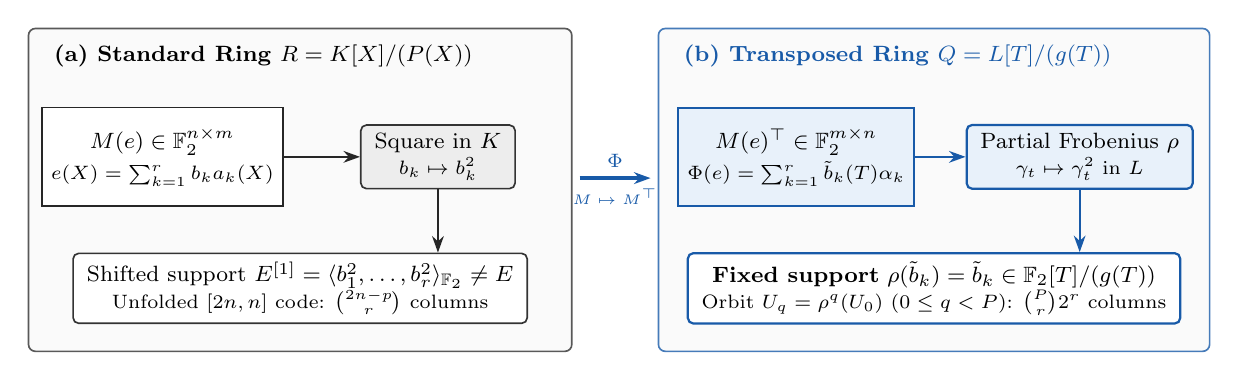
\begin{tikzpicture}[
    font=\footnotesize,
    panel/.style={draw=black!65, fill=gray!4, rounded corners=2.5pt, semithick},
    matbox/.style={draw=black!85, fill=white, semithick, minimum width=2.4cm, minimum height=1.25cm, align=center},
    accmat/.style={draw=accent, fill=accentlight, thick, minimum width=2.4cm, minimum height=1.25cm, align=center},
    pill/.style={draw=black!80, fill=gray!14, rounded corners=2pt, semithick, inner xsep=5pt, inner ysep=3pt, align=center},
    accpill/.style={draw=accent, fill=accentlight, rounded corners=2pt, thick, inner xsep=5pt, inner ysep=3pt, align=center},
    arr/.style={-{Stealth[length=2.1mm,width=1.5mm]}, semithick, color=black!85},
    accarr/.style={-{Stealth[length=2.1mm,width=1.5mm]}, semithick, color=accent}
]
    % Left Panel: Standard Ring R = K[X]/(P(X))
    \draw[panel] (-0.35, -1.75) rectangle (6.55, 2.35);
    \node[font=\footnotesize\bfseries, anchor=west] at (-0.15, 2.00) {(a) Standard Ring $R = K[X]/(P(X))$};

    \node[matbox] (Mstd) at (1.35, 0.72) {$M(e) \in \Ftwo^{n \times m}$\\[2pt]{\scriptsize $e(X) = \sum_{k=1}^r b_k a_k(X)$}};
    \node[pill] (Fstd) at (4.85, 0.72) {Square in $K$\\{\scriptsize $b_k \mapsto b_k^2$}};
    \node[pill, fill=white] (OutStd) at (3.10, -0.95) {Shifted support $E^{[1]} = \langle b_1^2,\dots,b_r^2\rangle_{\Ftwo} \neq E$\\{\scriptsize Unfolded $[2n, n]$ code: $\binom{2n-p}{r}$ columns}};

    \draw[arr] (Mstd.east) -- (Fstd.west);
    \draw[arr] (Fstd.south) -- (Fstd.south |- OutStd.north);

    % Center Transpose Arrow
    \draw[accarr, very thick] (6.65, 0.45) -- node[above, font=\scriptsize\bfseries] {$\Phi$} node[below, font=\tiny] {$M \mapsto M^\top$} (7.55, 0.45);

    % Right Panel: Transposed Ring Q = L[T]/(g(T))
    \draw[panel, draw=accent!80] (7.65, -1.75) rectangle (14.65, 2.35);
    \node[font=\footnotesize\bfseries, text=accent, anchor=west] at (7.85, 2.00) {(b) Transposed Ring $Q = L[T]/(g(T))$};

    \node[accmat] (Mtr) at (9.40, 0.72) {$M(e)^\top \in \Ftwo^{m \times n}$\\[2pt]{\scriptsize $\Phi(e) = \sum_{k=1}^r \tilde{b}_k(T)\alpha_k$}};
    \node[accpill] (Ftr) at (13.00, 0.72) {Partial Frobenius $\rho$\\{\scriptsize $\gamma_t \mapsto \gamma_t^2$ in $L$}};
    \node[accpill, fill=white] (OutTr) at (11.15, -0.95) {\textbf{Fixed support} $\rho(\tilde{b}_k) = \tilde{b}_k \in \Ftwo[T]/(g(T))$\\{\scriptsize Orbit $U_q = \rho^q(U_0)$ ($0 \le q < P$): $\binom{P}{r}2^r$ columns}};

    \draw[accarr] (Mtr.east) -- (Ftr.west);
    \draw[accarr] (Ftr.south) -- (Ftr.south |- OutTr.north);
\end{tikzpicture}
\caption{Comparison between (a) coefficient squaring in $R = K[X]/(P(X))$, which moves the unknown support $E \subset K$ to $E^{[1]} \neq E$, and (b) our transposed representation in $Q = L[T]/(g(T))$, where the partial Frobenius $\rho$ squares scalars in $L = \Ftwo[X]/(P(X))$ while fixing $\Phi(E) \subset \Ftwo[T]/(g(T))$ pointwise.}
\label{fig:transpose-frobenius}
\end{figure}

\subsection{Support Invariance Under Partial Frobenius}
Figure~\ref{fig:transpose-frobenius} illustrates how the transposed representation isolates the unknown support inside the fixed subring of the partial Frobenius automorphism $\rho$.

\begin{lemma}
\label{lem:transpose}
For $a = \sum_{j=0}^{n-1}(\sum_{t=0}^{m-1} \mu_{j,t} T^t) X^j \in R$, the transpose map
\[
    \Phi(a) \coloneqq \sum_{t=0}^{m-1} \left(\sum_{j=0}^{n-1} \mu_{j,t} X^j\right) T^t \in Q = L[T]/(g(T))
\]
is an $\Ftwo$-algebra isomorphism, and $\rho: Q \to Q$ defined by $\rho(\sum_{t=0}^{m-1} \gamma_t T^t) \coloneqq \sum_{t=0}^{m-1} \gamma_t^2 T^t$ ($\gamma_t \in L$) is a ring automorphism of order $n$ with fixed subring $Q^\rho = \Phi(K) = \Ftwo[T]/(g(T))$. For any $r$-dimensional subspace $E = \langle b_1, \dots, b_r \rangle_{\Ftwo} \subset K$:
\begin{enumerate}[leftmargin=1.8em,itemsep=2pt]
    \item $W \coloneqq \operatorname{span}_L(\Phi(E)) \subset Q$ is a free $L$-submodule of rank $r$ satisfying $W \cap \Phi(K) = \Phi(E)$.
    \item Setting $U_0 = \Phi(u)$, $H_0 = \Phi(h)$, $\tilde{b}_k = \Phi(b_k) \in Q^\rho$, and $\alpha_k = \Phi(a_k), \beta_k = \Phi(c_k) \in L$ for $e_1 = \sum_{k=1}^r b_k a_k$ and $e_2 = \sum_{k=1}^r b_k c_k$, applying $\rho^q$ ($q \ge 0$) to $u = e_1 + e_2 h$ yields
    \begin{equation}
    \label{eq:conj-orbit}
        U_q(T) = \sum_{k=1}^{r} \tilde{b}_k(T)\,\bigl(\alpha_k^{2^q} + H_q(T)\,\beta_k^{2^q}\bigr) \quad \text{in } Q, \qquad U_q = \rho^q(U_0),\; H_q = \rho^q(H_0).
    \end{equation}
\end{enumerate}
\end{lemma}

\begin{proof}
Both $R$ and $Q$ identify canonically with $\Ftwo[X, T]/(P(X), g(T))$; $\Phi$ exchanges the order of summation and is therefore a ring isomorphism. Because $\operatorname{char} L = 2$ and $g(T)$ has coefficients in $\Ftwo = L^{\sigma_L}$, squaring $L$-coefficients respects addition, multiplication, and reduction modulo $g(T)$, with fixed subring $\Ftwo[T]/(g(T)) = \Phi(K)$. In $Q = L \otimes_{\Ftwo} \Phi(K)$, $\Ftwo$-linearly independent elements $\tilde{b}_1, \dots, \tilde{b}_r \in \Phi(K)$ remain $L$-linearly independent, and expanding $\sum_{k=1}^r \lambda_k \tilde{b}_k \in \Phi(K)$ over an $\Ftwo$-basis of $L$ forces $\lambda_k \in \Ftwo$, proving $W \cap \Phi(K) = \Phi(E)$. Applying $\rho^q$ to $U_0 = \sum_{k=1}^r \tilde{b}_k(\alpha_k + H_0 \beta_k)$ fixes $\tilde{b}_k$ pointwise and squares $\alpha_k, \beta_k \in L$ $q$ times, yielding~\eqref{eq:conj-orbit}.
\end{proof}

\section{Ciphertext Support Recovery}
\label{sec:ct-attacks}

Given a public key $h$ and ciphertext syndrome $u = e_1 + e_2 h \bmod P(X)$ with error support $\dim_{\Ftwo} E = r$, we fix a window size $P \in \{r+1, \dots, n\}$ and evaluate~\eqref{eq:conj-orbit} for $0 \le q < P$. Table~\ref{tab:ct-variants} summarizes the four ciphertext support-recovery variants developed in this section.

\begin{table}[t]
\centering
\small
\caption{Summary of ciphertext support-recovery variants over $L = \Ftwo[X]/(P(X))$, where $\nu_L = \max(1, \binom{P}{r}2^r - \binom{P-1}{r}m)$ denotes the Stage~1 $L$-kernel dimension.}
\label{tab:ct-variants}
\setlength{\tabcolsep}{3.5pt}
\begin{tabular}{@{}llll@{}}
\toprule
\textbf{Variant} & \textbf{Threshold} & \textbf{Matrix Dimension Over $L$} & \textbf{Target Regime} \\
\midrule
Schur (Sec.~\ref{subsec:ct-schur}) & $m > 2^r,\; P = P_2^*$ & $\binom{P-1}{r}(m - 2^r) \times \binom{P-1}{r-1}2^r$ & $r \le 5$ dense Schur \\
Overdet.\ (Sec.~\ref{subsec:ct-overdet}) & $m > 2^r,\; P = P_1^*$ & $\binom{P-1}{r}m \times \binom{P}{r}2^r$ ($\nu_L = 1$)$^{\mathrm{a}}$ & Single-stage ($L$ only) \\
Sparse Krylov (Sec.~\ref{subsec:ct-sparse}) & $m > 2^r,\; P = P_2^*$ & $\binom{P-1}{r}m \times \binom{P}{r}2^r$ ($w = (r{+}1)2^r$) & $r = 6$ sparse Lanczos \\
Projection (Sec.~\ref{subsec:ct-split}) & $\deg P_1 \ge P_2^*$ & $\binom{P-1}{r}(m - 2^r) \times \binom{P-1}{r-1}2^r$ over $L_1$ & $X^n - 1$, $\gcd(m,n) > 1$ \\
\bottomrule
\end{tabular}
\\[0.3em]
{\scriptsize $^{\mathrm{a}}$Reduces to $\binom{P-1}{r}(m - 2^r) \times \binom{P-1}{r-1}2^r$ with $\nu_L = 1$ if local Schur elimination is applied before solving.}
\end{table}

\subsection{Ring-Valued Support-Minors Linearization}
\label{subsec:ct-plucker}

Following the Support-Minors cofactor strategy of Bardet et al.~\cite{BBC+20,BBGT23}, we eliminate the unknown basis elements $\tilde{b}_1, \dots, \tilde{b}_r \in Q^\rho$ by taking $(r+1) \times (r+1)$ determinants, but we carry out the expansion inside the commutative polynomial ring $Q = L[T]/(g(T))$ across the $P$ Frobenius conjugates rather than over an unfolded length-$2n$ code. Write $Z_{q,k}(T) \coloneqq \alpha_k^{2^q} + H_q(T)\beta_k^{2^q} \in Q$ and collect the $2P$ scalar columns in $L^r$ into the coordinate matrix
\[
    G \coloneqq \begin{pmatrix} A_0 & B_0 & \cdots & A_{P-1} & B_{P-1} \end{pmatrix} \in L^{r \times 2P}, \qquad
    A_{q,k} = \alpha_k^{2^q},\quad B_{q,k} = \beta_k^{2^q}.
\]
For any $(r+1)$-subset $S' \subseteq \{0, \dots, P-1\}$, the $(r+1)\times(r+1)$ matrix $M_{S'} = [U_q \mid Z_{q,1} \cdots Z_{q,r}]_{q \in S'}$ over $Q$ satisfies $M_{S'} (1, \tilde{b}_1, \dots, \tilde{b}_r)^\top = 0$, so $\det_Q(M_{S'}) = 0$. Expanding $\det_Q(M_{S'})$ along column~$0$ in characteristic~$2$ (where $+1 = -1$) gives
\[
    \sum_{a \in S'} U_a(T) \det_Q \bigl[A_s^\top + H_s(T) B_s^\top\bigr]_{s \in S' \setminus \{a\}} = 0 \quad \text{in } Q.
\]
By multilinearity of the determinant in each of the $r$ rows $s_1 < \dots < s_r$ of $S = S' \setminus \{a\}$, choosing either $A_{s_i}^\top$ ($\mu_i = 0$) or $H_{s_i}(T) B_{s_i}^\top$ ($\mu_i = 1$) in row~$i$ expands this $r \times r$ cofactor in $Q$ into $2^r$ terms:
\begin{equation}
\label{eq:laplace}
    E_{S'} \coloneqq \sum_{a \in S'} U_a(T) \, \gamma_{S' \setminus \{a\}}(T) = 0 \quad \text{in } Q,
    \qquad
    \gamma_S(T) \coloneqq \sum_{\mu \in \{0,1\}^r} p_{S,\mu} \prod_{\substack{i=1 \\ \mu_i = 1}}^{r} H_{s_i}(T),
\end{equation}
where $p_{S,\mu} \coloneqq \det_L G[:, (2 s_i + \mu_i)_{i=1}^r] \in L$ are the $N_{\text{col}} = \binom{P}{r} 2^r$ pair-transversal minors of $G$ selecting one column from each conjugate pair $\{A_{s_i}, B_{s_i}\}$ ($s_i \in S$). Extracting the $m$ coefficients of $1, T, \dots, T^{m-1}$ in~\eqref{eq:laplace} yields $m$ homogeneous $L$-linear equations per subset $S'$.

The next lemma lifts the standard MaxMinors pivot-syzygy reduction~\cite{BBC+20,BBGT23} from a field to the commutative ring $Q = L[T]/(g(T))$.

\begin{lemma}
\label{lem:row-complete}
If $U_0 \in Q^\times$, every equation $E_{S''}$ with $0 \notin S'' \subseteq \{1, \dots, P-1\}$ ($|S''| = r+1$) is a $Q$-linear combination of $\{E_{\{0\} \cup S} : S \subseteq \{1, \dots, P-1\},\, |S| = r\}$. Retaining only the $\binom{P-1}{r}$ subsets containing $0$ yields $N_{\text{row}} = \binom{P-1}{r} m$ scalar $L$-equations without changing the right kernel.
\end{lemma}

\begin{proof}
For any $r$-subset $S \subseteq \{1, \dots, P-1\}$, $E_{\{0\} \cup S} = 0$ rearranges in characteristic~$2$ to $U_0 \gamma_S = \sum_{x \in S} U_x \gamma_{\{0\} \cup (S \setminus \{x\})}$. Multiplying $E_{S''}$ by $U_0$ and substituting $S = S'' \setminus \{a\}$ gives
\[
    U_0 E_{S''} = \sum_{a \in S''} U_a (U_0 \gamma_{S'' \setminus \{a\}})
    = \sum_{a \in S''} \sum_{x \in S'' \setminus \{a\}} U_a U_x \, \gamma_{\{0\} \cup (S'' \setminus \{a, x\})} \equiv 0 \quad \text{in } Q,
\]
since each unordered pair $\{a, x\} \subset S''$ appears twice and cancels modulo~$2$. Because $U_0 \in Q^\times$, $E_{S''} = 0$.
\end{proof}

\subsection{Local Schur Elimination and Frobenius Threshold}
\label{subsec:ct-schur}

Partition the $\binom{P}{r}$ minor blocks of width $2^r$ into the $\binom{P-1}{r-1}$ core blocks with $0 \in S$ ($N'_{\text{col}} = \binom{P-1}{r-1}2^r$ columns) and the $K_{\text{blk}} = \binom{P-1}{r}$ non-pivot blocks with $0 \notin S$. In the $0$-anchored equation $E_{\{0\} \cup S_i} = U_0 \gamma_{S_i} + \sum_{x \in S_i} U_x \gamma_{\{0\} \cup (S_i \setminus \{x\})}$, every summand except $U_0 \gamma_{S_i}$ contains $0$ in its index set. Consequently, unlike systematic MaxMinors over a field where each non-pivot subset contributes a single scalar column, the $2^r$ columns of $S_i \subseteq \{1, \dots, P-1\}$ appear exclusively in the $i$-th $m$-row block $B_i \in L^{m \times 2^r}$:
\begin{equation}
\label{eq:block-staircase}
    \mathcal{M} = \begin{pmatrix}
        C_1 & B_1 & 0 & \cdots & 0 \\
        C_2 & 0 & B_2 & \cdots & 0 \\
        \vdots & \vdots & \vdots & \ddots & \vdots \\
        C_{K_{\text{blk}}} & 0 & 0 & \cdots & B_{K_{\text{blk}}}
    \end{pmatrix} \in L^{N_{\text{row}} \times N_{\text{col}}}, \qquad
    C_i \in L^{m \times N'_{\text{col}}},\quad B_i \in L^{m \times 2^r}.
\end{equation}
Figure~\ref{fig:schur-pipeline} illustrates the block-staircase structure of $\mathcal{M}$ and the resulting two-stage recovery pipeline.

\begin{figure}[t]
\centering
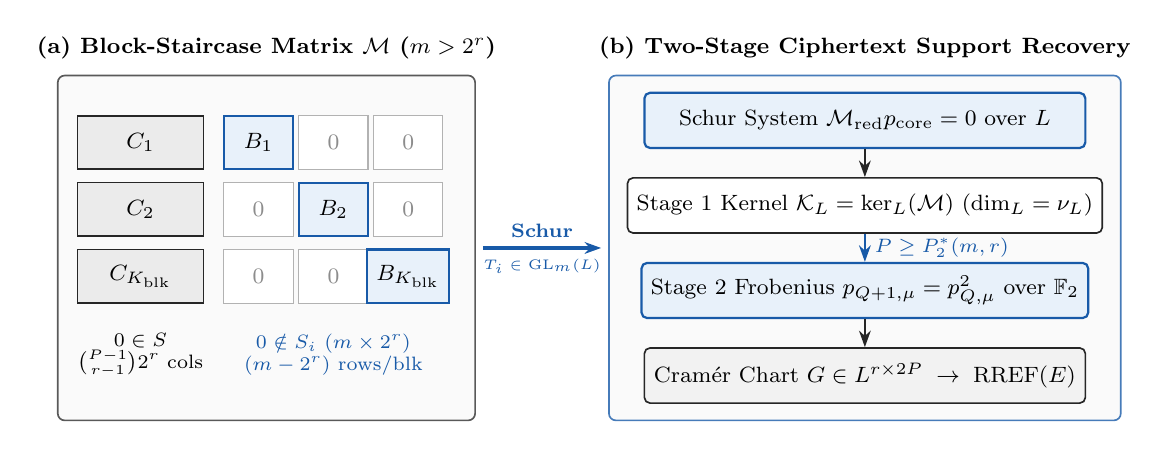
\begin{tikzpicture}[
    font=\footnotesize,
    panel/.style={draw=black!65, fill=gray!4, rounded corners=2.5pt, semithick},
    blkC/.style={draw=black!85, fill=gray!16, semithick, minimum width=1.60cm, minimum height=0.68cm, align=center},
    blkB/.style={draw=accent, fill=accentlight, thick, minimum width=0.88cm, minimum height=0.68cm, align=center},
    blkZ/.style={draw=black!30, fill=white, minimum width=0.88cm, minimum height=0.68cm, align=center, text=black!45},
    stage/.style={draw=black!85, fill=white, rounded corners=2pt, semithick, minimum width=5.6cm, minimum height=0.70cm, align=center},
    accstage/.style={draw=accent, fill=accentlight, rounded corners=2pt, thick, minimum width=5.6cm, minimum height=0.70cm, align=center},
    arr/.style={-{Stealth[length=2.1mm,width=1.5mm]}, semithick, color=black!85},
    accarr/.style={-{Stealth[length=2.1mm,width=1.5mm]}, semithick, color=accent}
]
    % Left: Block-staircase matrix M
    \node[font=\footnotesize\bfseries] at (2.40, 2.55) {(a) Block-Staircase Matrix $\mathcal{M}$ ($m > 2^r$)};
    \draw[panel] (-0.25, -2.18) rectangle (5.05, 2.20);

    % Row 1
    \node[blkC] (c1) at (0.80, 1.35) {$C_1$};
    \node[blkB] (b1) at (2.30, 1.35) {$B_1$};
    \node[blkZ] (z12) at (3.25, 1.35) {$0$};
    \node[blkZ] (z13) at (4.20, 1.35) {$0$};

    % Row 2
    \node[blkC] (c2) at (0.80, 0.50) {$C_2$};
    \node[blkZ] (z21) at (2.30, 0.50) {$0$};
    \node[blkB] (b2) at (3.25, 0.50) {$B_2$};
    \node[blkZ] (z23) at (3.25+0.95, 0.50) {$0$};

    % Row 3
    \node[blkC] (c3) at (0.80, -0.35) {$C_{K_{\text{blk}}}$};
    \node[blkZ] (z31) at (2.30, -0.35) {$0$};
    \node[blkZ] (z32) at (3.25, -0.35) {$0$};
    \node[blkB] (b3) at (4.20, -0.35) {$B_{K_{\text{blk}}}$};

    \node[font=\scriptsize, align=center] at (0.80, -1.35) {$0 \in S$\\$\binom{P-1}{r-1}2^r$ cols};
    \node[font=\scriptsize, text=accent, align=center] at (3.25, -1.35) {$0 \notin S_i$ ($m \times 2^r$)\\$(m - 2^r)$ rows/blk};

    % Center Schur Arrow
    \draw[accarr, very thick] (5.15, 0.01) -- node[above, font=\scriptsize\bfseries] {Schur} node[below, font=\tiny] {$T_i \in \GL_m(L)$} (6.65, 0.01);

    % Right: Two-stage pipeline
    \node[font=\footnotesize\bfseries] at (10.00, 2.55) {(b) Two-Stage Ciphertext Support Recovery};
    \draw[panel, draw=accent!80] (6.75, -2.18) rectangle (13.25, 2.20);

    \node[accstage] (st1) at (10.00, 1.63) {Schur System $\mathcal{M}_{\text{red}} p_{\text{core}} = 0$ over $L$};
    \node[stage]    (st2) at (10.00, 0.55) {Stage~1 Kernel $\mathcal{K}_L = \ker_L(\mathcal{M})$ ($\dim_L = \nu_L$)};
    \node[accstage] (st3) at (10.00, -0.53) {Stage~2 Frobenius $p_{Q+1,\mu} = p_{Q,\mu}^2$ over $\Ftwo$};
    \node[stage, fill=gray!10] (st4) at (10.00, -1.61) {Cram\'{e}r Chart $G \in L^{r \times 2P} \;\to\; \RREF(E)$};

    \draw[arr] (st1) -- (st2);
    \draw[accarr] (st2) -- node[right, font=\scriptsize] {$P \ge P_2^*(m,r)$} (st3);
    \draw[arr] (st3) -- (st4);
\end{tikzpicture}
\caption{Structure of the $0$-anchored Support-Minors system in $Q = L[T]/(g(T))$: (a) each non-pivot subset $S_i \subseteq \{1,\dots,P-1\}$ forms an isolated $m \times 2^r$ block $B_i$ that is eliminated locally with zero fill-in whenever $m > 2^r$; (b) the resulting two-stage solver extracts $\ker_L(\mathcal{M}_{\text{red}})$, enforces $p_{Q+1,\mu} = p_{Q,\mu}^2$ over $\Ftwo$, and reconstructs $G$ and $E$.}
\label{fig:schur-pipeline}
\end{figure}

\begin{proposition}
\label{prop:schur}
Suppose $m > 2^r$ and $\rk_L(B_i) = 2^r$ for all $1 \le i \le K_{\text{blk}}$. Left-multiplying row block $i$ by $T_i \in \GL_m(L)$ such that $T_i \begin{pmatrix} C_i & B_i \end{pmatrix} = \begin{pmatrix} \widetilde{C}_i & I_{2^r} \\ \mathcal{M}_{\text{red},i} & 0 \end{pmatrix}$ eliminates $B_1, \dots, B_{K_{\text{blk}}}$ locally with zero fill-in, yielding
\[
    \mathcal{M}_{\text{red}} = \begin{pmatrix} \mathcal{M}_{\text{red},1} \\ \vdots \\ \mathcal{M}_{\text{red},K_{\text{blk}}} \end{pmatrix} \in L^{N'_{\text{row}} \times N'_{\text{col}}}, \qquad
    N'_{\text{row}} = \binom{P-1}{r}(m - 2^r), \quad
    N'_{\text{col}} = \binom{P-1}{r-1} 2^r,
\]
with $\dim_L \ker(\mathcal{M}_{\text{red}}) = \dim_L \ker(\mathcal{M})$ and $N'_{\text{col}} - N'_{\text{row}} = N_{\text{col}} - N_{\text{row}}$.
\end{proposition}

\begin{proof}
Applying $\diag(T_1, \dots, T_{K_{\text{blk}}})$ to $\mathcal{M} p = 0$ decouples $p_{S_i} = \widetilde{C}_i p_{\text{core}}$ and leaves $\mathcal{M}_{\text{red}} p_{\text{core}} = 0$. By Pascal's identity $\binom{P}{r} - \binom{P-1}{r} = \binom{P-1}{r-1}$, we have $N'_{\text{col}} - N'_{\text{row}} = N_{\text{col}} - N_{\text{row}}$.
\end{proof}

When Stage~1 leaves kernel dimension $\nu_L = N_{\text{col}} - N_{\text{row}} > 1$ with basis $\{v^{(1)}, \dots, v^{(\nu_L)}\} \subset L^{N_{\text{col}}}$, Stage~2 enforces the Frobenius shift relation $A_{q+1} = A_q^{[1]}, B_{q+1} = B_q^{[1]}$ on minors:
\begin{equation}
\label{eq:frob-pin}
    p_{Q+1, \mu} = (p_{Q, \mu})^2 \qquad \forall\, Q \subseteq \{0, \dots, P-2\},\; |Q| = r,\; \mu \in \{0,1\}^r.
\end{equation}
Writing $p = \sum_{f=1}^{\nu_L} \theta_f v^{(f)}$ with $\theta_f = \sum_{j=0}^{n-1} \vartheta_{f,j} X^j \in L$ ($\vartheta_{f,j} \in \Ftwo$) turns~\eqref{eq:frob-pin} into a homogeneous $\Ftwo$-linear system $\mathcal{F} \vartheta = 0$ in $\nu_L n$ binary variables.

\begin{theorem}
\label{thm:ct-threshold}
On a Stage~1 kernel $\mathcal{K}_L = \ker_L(\mathcal{M})$ of rank $N_{\text{row}} = \binom{P-1}{r}m$, the Frobenius operator $\mathcal{F}|_{\mathcal{K}_L}$ satisfies $\binom{P-2}{r} m n$ $\Ftwo$-linear syzygies, so
\begin{equation}
\label{eq:frob-rank-bound}
    \rk_{\Ftwo}\!\left(\mathcal{F}\big|_{\mathcal{K}_L}\right) \le n \left[ \binom{P-1}{r} 2^r - \binom{P-2}{r} m \right].
\end{equation}
Two-stage $\TSM$ determines a unique solution ($\dim_{\Ftwo} \ker(\mathcal{F}|_{\mathcal{K}_L}) = 1$ when $\nu_L > 1$, or $\nu_L = 1$ up to $L^\times$) if and only if $m > 2^r$ and
\begin{equation}
\label{eq:p2-star}
    P \ge P_2^*(m, r) \coloneqq \left\lceil \frac{m r - 2^r}{m - 2^r} \right\rceil \le n,
\end{equation}
with strict inequality $m(P - r) > 2^r(P - 1)$ when requiring positive excess rank over $\Ftwo$.
\end{theorem}

\begin{proof}
For each of the $\binom{P-2}{r}$ subsets $S' \subseteq \{0, \dots, P-2\}$ containing $0$ and any $p \in \mathcal{K}_L$, Lemma~\ref{lem:row-complete} gives $E_{S'+1}(p) = 0$ in addition to $\rho(E_{S'}(p)) = 0$. Subtracting the two identities yields
\[
    \sum_{a \in S'} U_{a+1}(T) \sum_{\mu \in \{0,1\}^r} (p_{Q_a+1,\mu} + p_{Q_a,\mu}^2) \prod_{\mu_i = 1} H_{(Q_a)_i + 1}(T) \equiv 0 \quad \text{in } Q \qquad (Q_a = S' \setminus \{a\}),
\]
which imposes $\binom{P-2}{r} m n$ linear dependencies over $\Ftwo$ among the $\binom{P-1}{r} 2^r n$ bit-components of $(p_{Q+1,\mu} + p_{Q,\mu}^2)$ and proves~\eqref{eq:frob-rank-bound}. Because~\eqref{eq:frob-pin} restricts $L^\times$-scaling to $\lambda^2 = \lambda$ ($\lambda = 1$), unique recovery requires $n[\binom{P-1}{r}2^r - \binom{P-2}{r}m] \ge n[\binom{P}{r}2^r - \binom{P-1}{r}m]$, which simplifies via Pascal's identity to $\binom{P-2}{r-1} m \ge \binom{P-1}{r-1} 2^r$, or equivalently $m(P - r) \ge 2^r(P - 1)$ and~\eqref{eq:p2-star}.
\end{proof}

\paragraph{Reconstructing $G$ and $E$ from Pair-Transversal Minors.}
Once the minor vector $p$ is known, we adapt the chart-normalization procedure of~\cite{BBC+20,BBGT23} to our pair-transversal minors $(p_{S,\mu})$. Choose a non-singular chart (for instance $B_0, \dots, B_{r-1}$, corresponding to $S_0 = \{0, \dots, r-1\}$ and $\mu_0 = 1^r$) and normalize $G$ under its left $\GL_r(L)$-action so that $[B_0 \cdots B_{r-1}] = I_r$. Every column $c = 2q + \mu$ outside pairs $0, \dots, r-1$ ($q \ge r$) and every diagonal entry $A_{i,i}$ ($0 \le i < r$) is recovered by a single-column Cram\'{e}r replacement in $I_r$:
\[
    G_{i, 2q+\mu} = \frac{p_{\text{chart}(i \leftarrow 2q+\mu)}}{p_{S_0, 1^r}} \quad (q \ge r), \qquad
    A_{i, i} = \frac{p_{S_0, 1^r \oplus e_i}}{p_{S_0, 1^r}} \quad (0 \le i < r).
\]
For off-diagonal entries $A_{i, k}$ ($k \neq i$, $0 \le i, k < r$), pick any external column $v = G[:, 2q+\mu]$ ($q \ge r$) with $v_i \neq 0$; replacing columns $i$ and $k$ of $I_r$ by $A_i$ and $v$ gives a $2 \times 2$ determinant $p / p_{S_0, 1^r} = A_{i,i} v_k + A_{i,k} v_i$, whence $A_{i,k} = (p / p_{S_0, 1^r} + A_{i,i} v_k) / v_i$. Solving $r$ independent rows of~\eqref{eq:conj-orbit} over $Q$ then yields $(\tilde{b}_1, \dots, \tilde{b}_r)$ and $E = \RREF(\Supp(\Phi^{-1}(\tilde{b})))$ (Algorithm~3).

\begin{figure}[t]
\centering
\renewcommand{\arraystretch}{1.12}
\begin{tabular}{@{}>{\raggedright\arraybackslash}p{\textwidth}@{}}
\toprule
\textbf{Algorithm 3:} Two-Stage Ciphertext Support Recovery ($m > 2^r$, $P = P_2^*(m,r) \le n$) \\
\midrule
\algstep{1}{Compute $U_q = \rho^q(\Phi(u))$ and $H_q = \rho^q(\Phi(h))$ in $Q = L[T]/(g(T))$ for $0 \le q < P$.} \\
\algstep{2}{For each $r$-subset $S_i \subseteq \{1, \dots, P-1\}$, form $\begin{pmatrix} C_i & B_i \end{pmatrix}$ from $E_{\{0\} \cup S_i}$ and eliminate $B_i$ into $\mathcal{M}_{\text{red}, i}$.} \\
\algstep{3}{Compute $\ker_L(\mathcal{M}_{\text{red}})$ of dimension $\nu_L$ and back-substitute $p_{S_i} = \widetilde{C}_i p_{\text{core}}$.} \\
\algstep{4}{If $\nu_L > 1$, solve $p_{Q+1,\mu} + p_{Q,\mu}^2 = 0$ over $\Ftwo$ on $\ker_L(\mathcal{M})$ to obtain $p$.} \\
\algstep{5}{Normalize a non-singular chart $[B_0 \cdots B_{r-1}] = I_r$ and reconstruct $G \in L^{r \times 2P}$ via Cram\'{e}r minor ratios.} \\
\algstep{6}{Solve $[G_{k, 2q} + H_q G_{k, 2q+1}]_{q \in I,\, 1 \le k \le r} \cdot \tilde{b} = (U_q)_{q \in I}$ over $Q$ ($|I|=r$); set $E \leftarrow \RREF(\Supp(\Phi^{-1}(\tilde{b})))$.} \\
\algstep{7}{In CCA2 mode, set $\mu' = v \oplus \SHA(E)$, verify $\SHA(\mu') = d_{\text{tag}}$, and \textbf{return} $\SHA(\mu' \parallel u \parallel v)$.} \\
\bottomrule
\end{tabular}
\end{figure}

\subsection{Overdetermined Single-Stage Recovery}
\label{subsec:ct-overdet}

\begin{corollary}
\label{cor:p1-star}
For $m > 2^r$, choosing $P \ge P_1^*(m, r) \coloneqq \lceil m r / (m - 2^r) \rceil \le n$ (or $m r / (m - 2^r) + 1$ when $(m - 2^r) \mid m r$) gives $N_{\text{row}} \ge N_{\text{col}} - 1$ and $\nu_L = \dim_L \ker(\mathcal{M}_{\text{red}}) = 1$, recovering $p$ up to $L^\times$-scaling in Stage~1 without forming the binary Frobenius matrix $\mathcal{F}$.
\end{corollary}

On $\mathsf{LOCKER\text{-}I}$ $(m=71, n=83, r=5)$, setting $P = P_1^*(71, 5) = 10$ gives an unreduced $8{,}946 \times 8{,}064$ system ($4{,}914 \times 4{,}032$ after local Schur reduction) of rank $N_{\text{col}} - 1$ ($\nu_L = 1$). On $r = 6, m = 107$ ($\mathsf{LOCKER\text{-}III/VI}$), increasing $P$ from $P_2^* = 14$ to $P_1^* = 15$ eliminates the Stage~2 binary matrix of $869\text{--}1{,}164\text{ GiB}$ altogether.

\subsection{Sparse Krylov Solving}
\label{subsec:ct-sparse}

At $r = 6$, dense storage of the unreduced matrix $\mathcal{M}$ requires $565\text{--}863\text{ GB}$ of memory ($97\text{--}508\text{ GB}$ after local Schur reduction). Retaining the unreduced matrix $\mathcal{M}$ in~\eqref{eq:block-staircase} preserves exact constant row weight for sparse Krylov solvers such as Wiedemann~\cite{Wiedemann86} and Block-Lanczos~\cite{Montgomery95}.

\begin{proposition}
\label{prop:sparse}
Every row of $\mathcal{M} \in L^{N_{\text{row}} \times N_{\text{col}}}$ contains at most $w = (r + 1) 2^r$ non-zero entries across the $r + 1$ disjoint $2^r$-column blocks $S' \setminus \{a\}$ ($a \in S'$). Compressed sparse row ($\mathsf{CSR}$) storage uses $N_{\text{row}} w (4 + 8 \lceil n/64 \rceil) + 8(N_{\text{row}} + 1)$ bytes, and Block-Lanczos on $\mathcal{M}^\top \mathcal{M}$ followed by Stage~2 requires
\begin{equation}
\label{eq:sparse-gates}
    C_{\text{CT}}(m, n, r) = 4 N_{\text{col}} N_{\text{row}} w n^2 + \frac{(\nu_L n)^{\omega_0}}{7} + \binom{P-1}{r} 2^r \nu_L n^2 \quad \text{gates} \quad (\omega_0 = \log_2 7),
\end{equation}
at $2 n^2$ two-input gates per $\F_{2^n}$ multiply-accumulate.
\end{proposition}

\begin{proof}
For fixed $S' = \{0\} \cup S$, the $r + 1$ subsets $S' \setminus \{a\}$ ($a \in S'$) are distinct, so their $2^r$-column blocks do not overlap. Block-Lanczos~\cite{Montgomery95} with block width $\beta$ performs $\lceil N_{\text{col}}/\beta \rceil$ iterations of $\beta$-wide multiplications by $\mathcal{M}$ and $\mathcal{M}^\top$, totaling $2 N_{\text{col}} N_{\text{row}} w$ scalar $\F_{2^n}$ multiply-adds ($4 N_{\text{col}} N_{\text{row}} w n^2$ gates), plus $\Ftwo$ elimination on $\nu_L n$ columns.
\end{proof}

\subsection{Reducible Quotients and Non-Coprime Degrees}
\label{subsec:ct-split}

\begin{proposition}
\label{prop:split-ring}
\begin{enumerate}[leftmargin=1.8em,itemsep=2pt]
    \item If $P(X) \in \Ftwo[X]$ has an irreducible divisor $P_1(X) \mid P(X)$ of degree $n_1 \ge P_2^*(m, r)$ (in particular, the cyclotomic polynomial $\Phi_n(X)$ of degree $n - 1$ inside $X^n - 1 = (X+1)\Phi_n(X)$ when $\operatorname{ord}_n(2) = n - 1$), projecting to $K[X]/(P_1(X))$ and running $\TSM$ over $L_1 = \Ftwo[X]/(P_1(X))$ recovers $E$ with probability at least $1 - 2^{-(n_1 - r)}$. Running $\TSM$ on $K[X]/(X^n - 1)$ directly fails because $\rho = \operatorname{id}$ on $K[X]/(X+1)$ produces identical rows in $M_{S'}$.
    \item If $P(X)$ is $\Ftwo$-irreducible and $k = \gcd(m, n) > 1$, then $Q \cong (\F_{2^{\lcm(m,n)}})^k$ contains zero divisors, yet $L = \F_{2^n}$ remains a field, $(L \otimes_{\Ftwo} E) \cap \Phi(K) = \Phi(E)$, and~\eqref{eq:laplace}--\eqref{eq:frob-pin} hold over $L$ and $\Ftwo$ whenever $U_0 \in Q^\times$ (which occurs with probability $(1 - 2^{-\lcm(m,n)})^k$).
\end{enumerate}
\end{proposition}

\begin{proof}
In~(1), the natural projection $\pi_1: R \twoheadrightarrow K[X]/(P_1(X))$ is $K$-linear, so $\Supp(\pi_1(e_i)) \subseteq E$ and $\pi_1(e_2)$ has full rank $r$ modulo $\Phi_n(X)$ whenever $(e_{2,j} + e_{2,n-1})_{0 \le j < n-1}$ spans $E$. In~(2), Laplace expansion holds over any commutative ring $Q$, while all entries of $\mathcal{M}$ and $\mathcal{F}$ lie in the fields $L$ and $\Ftwo$.
\end{proof}

\section{Public-Key Secret Recovery}
\label{sec:pk-attacks}

In $\mathsf{LOCKER}$, $\mathsf{ROLLO\text{-}I}$, and $\mathsf{ROLLO\text{-}II}$, the public key $h = x^{-1} y \bmod P(X)$ satisfies the homogeneous rank-$d$ relation
\[
    x(X)\, h(X) + y(X) \equiv 0 \pmod{P(X)}, \qquad \Supp(x), \Supp(y) \subseteq F = \langle f_1, \dots, f_d \rangle_{\Ftwo} \subset K.
\]
Recovering any nonzero $K^\times$-multiple $(\gamma F, \gamma x, \gamma y)$ ($\gamma \in K^\times$) yields a functionally equivalent secret key for decapsulation. (For $\mathsf{ROLLO\text{-}III}$, where $h \xleftarrow{\$} R$ is uniform and $\mathsf{pk} = (h, s = x + h y \bmod P(X))$ is inhomogeneous of secret rank $d = w$, Algorithm~3 of Section~\ref{sec:ct-attacks} applies directly to $(h, s)$ to recover $(F, x, y)$.)

\subsection{Principal Minors From Partial-Frobenius Products}
\label{subsec:pk-closed}

Write $\Phi(x) = \sum_{k=1}^d \tilde{f}_k(T) \alpha_k$ and $\Phi(y) = \sum_{k=1}^d \tilde{f}_k(T) \beta_k$ ($\tilde{f}_k \in Q^\rho$, $\alpha_k, \beta_k \in L$). Applying $\rho^q$ for $0 \le q < d$ gives $d$ homogeneous equations in $Q$:
\begin{equation}
\label{eq:pk-homog}
    \sum_{k=1}^{d} \tilde{f}_k(T)\,\bigl(\alpha_k^{2^q} H_q(T) + \beta_k^{2^q}\bigr) = 0 \quad \text{in } Q \qquad (0 \le q < d).
\end{equation}
Define the Moore matrices $A = (\alpha_k^{2^q})_{0 \le q < d,\, 1 \le k \le d} \in \GL_d(L)$ and $B = (\beta_k^{2^q})_{0 \le q < d,\, 1 \le k \le d} \in \GL_d(L)$ (both invertible because $\rk_{\Ftwo}(x) = \rk_{\Ftwo}(y) = d$), and set $M \coloneqq B A^{-1} \in \GL_d(L)$.

\begin{theorem}
\label{thm:pk-minors}
Let $C_H \in L^{m \times 2^d}$ be the matrix whose column $\mu \in \{0,1\}^d$ holds the $m$ $T$-coefficients of $\prod_{q:\,\mu_q = 1} H_q(T) \in Q$. Every valid keypair $(x, y)$ defines a right kernel vector $p \in \ker_L(C_H)$ with $p_{1\dots 1} = \det(A) \neq 0$ and
\[
    \frac{p_\mu}{p_{1\dots 1}} = \Delta_{Z(\mu)}(M) \coloneqq \det M[Z(\mu), Z(\mu)], \qquad Z(\mu) \coloneqq \{0 \le q < d : \mu_q = 0\}.
\]
When $m \ge 2^d$, $C_H$ has generic rank $2^d - 1$, so one $m \times 2^d$ elimination over $L$ yields all $2^d$ principal minors of $M$.
\end{theorem}

\begin{proof}
Since $\tilde{f}_1, \dots, \tilde{f}_d$ are $L$-linearly independent,~\eqref{eq:pk-homog} implies $\det_Q[\alpha_k^{2^q} H_q(T) + \beta_k^{2^q}] = 0$. Expanding row $q$ into $\mu_q = 1$ ($\alpha_k^{2^q} H_q$) and $\mu_q = 0$ ($\beta_k^{2^q}$) gives $C_H p = 0$, where $p_\mu = \det N_\mu$ takes row $q$ from $A$ if $\mu_q = 1$ and from $B = M A$ if $\mu_q = 0$. Right-multiplying $N_\mu$ by $A^{-1}$ places unit rows $e_q^\top$ at $q \notin Z(\mu)$ and rows of $M$ at $q \in Z(\mu)$, giving $\det(N_\mu A^{-1}) = \det M[Z(\mu), Z(\mu)]$.
\end{proof}

\subsection{Closed-Form Moore-Matrix Gauge Recursion}
\label{subsec:pk-moore}

Once all $2^d$ principal minors $\Delta_Z(M)$ are extracted from $\ker_L(C_H)$, the classical PMAP reduction~\cite{Loewy86,GT06} reconstructs a representative $\tilde{M}$ up to diagonal conjugation $M = D \tilde{M} D^{-1}$ ($D = \diag(D_0, \dots, D_{d-1}) \in (L^\times)^d$) and transposition $\tilde{M} \leftrightarrow \tilde{M}^\top$. Imposing the row-$0$ gauge $\tilde{M}_{0,j} = 1$ ($1 \le j < d$) immediately gives the diagonal $\tilde{M}_{i,i} = \Delta_{\{i\}}$, the $2$-cycle products $\pi_{i,j} \coloneqq M_{i,j}M_{j,i} = \Delta_{\{i\}}\Delta_{\{j\}} + \Delta_{\{i,j\}}$, and column~$0$ as $\tilde{M}_{j,0} = \pi_{0,j}$. Expanding any $3 \times 3$ principal minor $\Delta_{\{i,j,k\}}$ isolates the $3$-cycle sum
\[
    \tilde{M}_{i,j}\tilde{M}_{j,k}\tilde{M}_{k,i} + \tilde{M}_{i,k}\tilde{M}_{k,j}\tilde{M}_{j,i} = T_{i,j,k} \coloneqq \Delta_{\{i,j,k\}} + \Delta_{\{i\}}\Delta_{\{j\}}\Delta_{\{k\}} + \Delta_{\{i\}}\pi_{j,k} + \Delta_{\{j\}}\pi_{i,k} + \Delta_{\{k\}}\pi_{i,j}.
\]
Setting $(i, j, k) = (0, 1, j)$ ($2 \le j < d$) with $\tilde{M}_{0,1} = \tilde{M}_{0,j} = 1$ and $\tilde{M}_{j,1} = \pi_{1,j}/\tilde{M}_{1,j}$ yields $d - 2$ univariate quadratics $\pi_{0,j} \tilde{M}_{1,j}^2 + T_{0,1,j} \tilde{M}_{1,j} + \pi_{0,1}\pi_{1,j} = 0$ over $L$ (solved via half-traces for odd $n$). Once row~$1$ and column~$1$ are fixed, $(T_{0,i,j}, T_{1,i,j})$ form a $2 \times 2$ linear system in $(\tilde{M}_{i,j}, \tilde{M}_{j,i})$ for every $2 \le i < j < d$, leaving at most two consistent candidates $\{\tilde{M}, \tilde{M}^\top\}$.

In a general PMAP instance, the diagonal gauge $D \in (L^\times)^d$ cannot be recovered from principal minors alone. Theorem~\ref{thm:moore-rec} resolves this gauge ambiguity in closed form without searching $(L^\times)^{d-1}$ by exploiting the Frobenius row-shift structure of the Moore matrices $A$ and $B$.

\begin{theorem}
\label{thm:moore-rec}
For Moore matrices $A_{i,k} = \alpha_k^{2^i}$ and $B_{i,k} = \beta_k^{2^i} = (M A)_{i,k}$ with $M = D \tilde{M} D^{-1}$ and $\tilde{M}_{0,j} = 1$ ($j \ge 1$), rescaling $(x, y) \mapsto (\delta x, \delta y)$ ($\delta \in L^\times$) fixes $D_0 = D_1 = 1$, and $D_2, \dots, D_{d-1}$ satisfy
\begin{equation}
\label{eq:moore-recursion}
    D_{i+1} = D_i^2 \cdot \frac{\tilde{M}_{1,0}\,\tilde{M}_{i,d-1}^2}{\tilde{M}_{0,d-1}^2\,\tilde{M}_{i+1,0}} \qquad (1 \le i \le d - 2).
\end{equation}
The secret subspace $\langle \alpha_1, \dots, \alpha_d \rangle_{\Ftwo} \subset L$ equals $\ker_{\Ftwo}(\mathcal{L}_\alpha)$ for
\begin{equation}
\label{eq:L-alpha}
    \mathcal{L}_\alpha(Z) = Z^{2^d} + \sum_{j=1}^{d-1} \frac{M_{0,j-1}^2 + M_{1,j}}{M_{0,d-1}^2}\, Z^{2^j} + \frac{M_{1,0}}{M_{0,d-1}^2}\, Z,
\end{equation}
with total gate complexity $C_{\text{PK}}(m, n, d) = (2^d - d - 1) \cdot 2 m^2 n^2 + m \cdot 2^{2d} n^2 + \frac{1}{2} d^2 m^3 n$.
\end{theorem}

\begin{proof}
Squaring row~$i$ of $B = M A$ ($0 \le i \le d - 2$) gives $\beta_k^{2^{i+1}} = M_{i,d-1}^2 \alpha_k^{2^d} + \sum_{j=1}^{d-1} M_{i,j-1}^2 \alpha_k^{2^j}$, whereas row~$i+1$ of $B = M A$ gives $\beta_k^{2^{i+1}} = \sum_{j=0}^{d-1} M_{i+1,j} \alpha_k^{2^j}$. Subtracting the two expressions shows that
\[
    \mathcal{L}^{(i)}(Z) \coloneqq Z^{2^d} + \sum_{j=1}^{d-1} \frac{M_{i,j-1}^2 + M_{i+1,j}}{M_{i,d-1}^2}\, Z^{2^j} + \frac{M_{i+1,0}}{M_{i,d-1}^2}\, Z
\]
vanishes on $V_\alpha = \langle \alpha_1, \dots, \alpha_d \rangle_{\Ftwo}$ for every $0 \le i \le d - 2$ ($M_{i,d-1} \neq 0$ since $|V_\alpha| = 2^d$). Because the monic degree-$2^d$ annihilator $\prod_{v \in V_\alpha}(Z + v)$ is unique, $\mathcal{L}^{(i)} = \mathcal{L}^{(0)}$ for all $i$, so $M_{i+1,0} / M_{i,d-1}^2 = M_{1,0} / M_{0,d-1}^2$. Rescaling $(\alpha_k, \beta_k) \mapsto (\delta \alpha_k, \delta \beta_k)$ maps $D_i \mapsto \delta^{2^i - 1} D_i$, so $\delta = D_1^{-1}$ sets $D_0 = D_1 = 1$. Substituting $M_{i,j} = (D_i / D_j) \tilde{M}_{i,j}$ gives
\[
    \frac{(D_{i+1}/D_0)\,\tilde{M}_{i+1,0}}{(D_i / D_{d-1})^2\,\tilde{M}_{i,d-1}^2}
    = \frac{(D_1 / D_0)\,\tilde{M}_{1,0}}{(D_0 / D_{d-1})^2\,\tilde{M}_{0,d-1}^2},
\]
where $D_{d-1}^2$ cancels from both denominators, yielding~\eqref{eq:moore-recursion} and~\eqref{eq:L-alpha} (Algorithm~4).
\end{proof}

\begin{figure}[t]
\centering
\renewcommand{\arraystretch}{1.12}
\begin{tabular}{@{}>{\raggedright\arraybackslash}p{\textwidth}@{}}
\toprule
\textbf{Algorithm 4:} Direct Public-Key Secret Recovery ($m \ge 2^d$) \\
\midrule
\algstep{1}{Compute $H_q = \rho^q(\Phi(h))$ ($0 \le q < d$) and form $C_H \in L^{m \times 2^d}$ with columns $\prod_{\mu_q=1} H_q(T)$.} \\
\algstep{2}{Find $p \in \ker_L(C_H) \setminus \{0\}$ and normalize $\Delta_{Z(\mu)} \leftarrow p_\mu / p_{1\dots 1}$ for all $\mu \in \{0,1\}^d$.} \\
\algstep{3}{Reconstruct $\tilde{M}$ ($\tilde{M}_{0,j}=1$) from the $d-2$ quadratics on $(0,1,j)$ and $2 \times 2$ linear systems on $(0,i,j),(1,i,j)$.} \\
\algstep{4}{For $\hat{M} \in \{\tilde{M}, \tilde{M}^\top\}$ (re-gauged to $\hat{M}_{0,j}=1$), compute $D$ via~\eqref{eq:moore-recursion}, $M = D \hat{M} D^{-1}$, $\langle \alpha_1, \dots, \alpha_d \rangle_{\Ftwo} = \ker_{\Ftwo}(\mathcal{L}_\alpha)$ via~\eqref{eq:L-alpha}, and $\beta = M_{0,\cdot} A$; solve $\sum_{k=1}^d \tilde{f}_k(T)(\alpha_k H_0(T) + \beta_k) = 0$ over $\Ftwo$ and \textbf{return} $\Phi^{-1}(\tilde{f}, \Phi(x), \Phi(y))$.} \\
\bottomrule
\end{tabular}
\end{figure}

\subsection{Transposed Subspace Search for Small Field Degrees}
\label{subsec:pk-window}

When $m < 2^d$, $C_H \in L^{m \times 2^d}$ has an underdetermined kernel of dimension at least $2^d - m > 1$. In this regime, the classical structural dual-LRPC subspace search~\cite{GMRZ13,HT15,ROLLO20} tests whether a candidate $D$-dimensional subspace $W \subset K$ ($d \le D < m$) contains a $K^\times$-multiple $\gamma F$ of the secret support by solving an $n(m - D) \times n D$ binary system in $O((m - D)D^2 n^3)$ bit operations. Working over the field $L = \Ftwo[X]/(P(X))$ reduces each window test by a factor of $n$ to an $(m - D) \times D$ matrix over $L$, while confirming that the exponential Grassmannian covering factor keeps $m < 2^d$ parameters secure.

\begin{proposition}
\label{prop:window}
Let $W \subset K$ be a $D$-dimensional $\Ftwo$-subspace ($d \le D < m$) extended to a basis $(w_0, \dots, w_{m-1})$ of $K$ with $\Ftwo$-dual basis $(\omega_0, \dots, \omega_{m-1})$, and define $M_W \in L^{(m - D) \times D}$ by
\[
    (M_W)_{k, j} \coloneqq \sum_{i=0}^{n-1} \langle \omega_{D+k},\, w_j h_i \rangle \, X^i \in L \qquad (0 \le k < m - D,\; 0 \le j < D).
\]
Then $\ker_L(M_W) \cong \{x \in R : \Supp(x) \subseteq W \text{ and } \Supp(x h) \subseteq W\}$. One $O((m - D) D^2 n^2)$ elimination over $L$ tests whether $\gamma F \subseteq W$ for any $\gamma \in K^\times$, covering a multiplicative orbit of size $2^m - 1$; covering the full keyspace requires at least $\genfrac{[}{]}{0pt}{}{m}{d}_2 \big/ \bigl((2^m - 1)\genfrac{[}{]}{0pt}{}{D}{d}_2\bigr)$ subspaces ($\ge 2^{406.8}$ at $D = 8$, $\ge 2^{397.8}$ at $D = 9$, and $\ge 2^{205.0}$ at $D = 33$ on $2020$ $\mathsf{ROLLO\text{-}I\text{-}128}$).
\end{proposition}

\begin{proof}
Every $x \in R$ with $\Supp(x) \subseteq W$ writes uniquely as $x = \sum_{j=0}^{D-1} w_j \lambda_j(X)$ ($\lambda_j \in L$), and its $w_{D+k}$-component after multiplying by $h \bmod P(X)$ equals $\sum_{j=0}^{D-1} (M_W)_{k,j} \lambda_j$. If $\gamma F \subseteq W$, then $\gamma x \in \ker_L(M_W) \setminus \{0\}$. On $2020$ $\mathsf{ROLLO\text{-}I\text{-}128}$ $(m=67, n=83, d=8)$ at $D = 33$, a single $34 \times 33$ window test over $\F_{2^{83}}$ executes in $0.29\text{ s}$ on one core, but requires $\ge 2^{205.0}$ windows to cover $\Gr_{\Ftwo}(8, K)$.
\end{proof}

\section{Phase Transitions and Impossibility Barriers}
\label{sec:barriers}

\subsection{Exact Binary Nullity Below Threshold}
In the sub-threshold regime $m \le 2^r$ ($2019$ $\mathsf{ROLLO\text{-}I/II\text{-}256}$, $2020$ $\mathsf{ROLLO}$, and $\mathsf{new2ROLLO\text{-}I}$), neither increasing the number of Frobenius conjugates $P \le n$ nor adjoining quadratic Grassmannian Pl\"{u}cker relations closes the system.

\begin{theorem}
\label{thm:dichotomy}
Over $Q = L[T]/(g(T))$ with authentic conjugates $H_q = \rho^q(H_0)$ and $U_q = \rho^q(U_0)$:
\begin{enumerate}[leftmargin=1.8em,itemsep=2pt]
    \item Because $\rho$ is an automorphism of $Q$ fixing $\Phi(K)$ pointwise, equation~$q$ of~\eqref{eq:conj-orbit} is the $\rho^q$-image of equation~$0$. The solution set $\{E' \in \Gr_{\Ftwo}(r, K) : U_0 \in W_{E'} + H_0 W_{E'}\}$ is independent of $P$, with expected spurious count $\genfrac{[}{]}{0pt}{}{m}{r}_2 2^{-n(m - 2r)}$.
    \item Eliminating shifted variables via $p_{Q+1,\mu} = p_{Q,\mu}^2$ leaves $2^r \binom{P-1}{r-1} n$ binary unknowns, while $\binom{P-2}{r}$ of the $\binom{P-1}{r}$ $0$-anchored equations become redundant via $E_{S'+1} = \rho(E_{S'})$, leaving only the $\binom{P-2}{r-1}$ blocks with $\{0, 1\} \subseteq S'$. For all $m \le 2^r$ and $r+1 \le P \le n$ ($d > r$), the exact $\Ftwo$-nullity is
    \begin{equation}
    \label{eq:binary-nullity}
        \nu_{\Ftwo}(P) = n \left[ 2^r \binom{P-1}{r-1} - m \binom{P-2}{r-1} \right],
    \end{equation}
    which grows strictly with $P$.
\end{enumerate}
\end{theorem}

\begin{proof}
Part~(1) follows from bijectivity of $\rho^q$ on $Q$ and $\rho^q(\tilde{b}_k) = \tilde{b}_k$. For Part~(2), under $p_{Q+1,\mu} = p_{Q,\mu}^2$, every $r$-subset $Q \subseteq \{0, \dots, P-1\}$ is determined by the unique shifted subset $Q - \min Q \ni 0$ when anchored from below, or equivalently $Q + (P - 1 - \max Q) \ni P - 1$ within $\{0, \dots, P-1\}$; there are $\binom{P-1}{r-1}$ such orbits, giving $2^r \binom{P-1}{r-1} n$ independent binary variables. Among the $\binom{P-1}{r}$ $0$-anchored equations $E_{S'}$, every subset $S' \subseteq \{0, \dots, P-2\}$ containing $0$ ($\binom{P-2}{r}$ subsets) satisfies $\rho(E_{S'}) = E_{S'+1}$, which already lies in the $Q$-span of $\{E_{\{0\}\cup S}\}$ by Lemma~\ref{lem:row-complete}. Subtracting these $\binom{P-2}{r}$ redundant $Q$-equations leaves $\binom{P-1}{r} - \binom{P-2}{r} = \binom{P-2}{r-1}$ independent $Q$-equations ($mn$ bits each), yielding~\eqref{eq:binary-nullity}. When $m \le 2^r$, $\nu_{\Ftwo}(P+1) - \nu_{\Ftwo}(P) = n[2^r\binom{P-1}{r-2} - m\binom{P-2}{r-2}] > 0$.
\end{proof}

\subsection{Quadratic Pl\"{u}cker Deficit and Scope Boundaries}
\begin{table}[t]
\centering
\caption{Exact binary nullity $\nu_{\Ftwo}(P)$ and quadratic Grassmannian Pl\"{u}cker relation deficit across representative $m \le 2^r$ parameter sets. Here $\binom{\nu_{\Ftwo}+1}{2}$ counts quadratic binary monomials on the kernel, and $N_{\text{Pl}} = \binom{2P}{r-1}\binom{2P-r+1}{r+1}$ counts quadratic Pl\"{u}cker generators over $L$.}
\label{tab:deg2-deficit}
\setlength{\tabcolsep}{4.8pt}
\begin{tabular}{@{}lcccccc@{}}
\toprule
\textbf{Parameter Set} & \textbf{$(m, n, r)$} & \textbf{$P$} & \textbf{$\nu_{\Ftwo}(P)$} & \textbf{$\binom{\nu_{\Ftwo}+1}{2}$} & \textbf{$N_{\text{Pl}}$} & \textbf{$n N_{\text{Pl}}$} \\
\midrule
$2019$ $\mathsf{ROLLO\text{-}I\text{-}256}$ & $(113, 67, 7)$ & $7$ & $8.58{\times}10^3$ & $3.68{\times}10^7$ & $3.00{\times}10^3$ & $2.01{\times}10^5$ \\
$2019$ $\mathsf{ROLLO\text{-}II\text{-}256}$ & $(127, 157, 7)$ & $9$ & $4.23{\times}10^5$ & $8.95{\times}10^{10}$ & $9.19{\times}10^6$ & $1.44{\times}10^9$ \\
$2020$ $\mathsf{ROLLO\text{-}I\text{-}128}$ & $(67, 83, 7)$ & $8$ & $6.88{\times}10^4$ & $2.37{\times}10^9$ & $3.60{\times}10^5$ & $2.99{\times}10^7$ \\
$2020$ $\mathsf{ROLLO\text{-}I\text{-}192}$ & $(79, 97, 8)$ & $8$ & $2.48{\times}10^4$ & $3.08{\times}10^8$ & $1.14{\times}10^4$ & $1.11{\times}10^6$ \\
$2020$ $\mathsf{ROLLO\text{-}I\text{-}256}$ & $(97, 113, 9)$ & $9$ & $5.79{\times}10^4$ & $1.67{\times}10^9$ & $4.38{\times}10^4$ & $4.94{\times}10^6$ \\
$2020$ $\mathsf{ROLLO\text{-}II\text{-}128}$ & $(83, 189, 7)$ & $8$ & $1.54{\times}10^5$ & $1.18{\times}10^{10}$ & $3.60{\times}10^5$ & $6.81{\times}10^7$ \\
$2020$ $\mathsf{ROLLO\text{-}II\text{-}192}$ & $(97, 193, 8)$ & $8$ & $4.94{\times}10^4$ & $1.22{\times}10^9$ & $1.14{\times}10^4$ & $2.21{\times}10^6$ \\
$2020$ $\mathsf{ROLLO\text{-}II\text{-}256}$ & $(97, 211, 8)$ & $9$ & $4.12{\times}10^5$ & $8.47{\times}10^{10}$ & $1.75{\times}10^6$ & $3.69{\times}10^8$ \\
$\mathsf{new2ROLLO\text{-}I\text{-}128}$~\cite{BBC+20} & $(73, 83, 7)$ & $8$ & $6.83{\times}10^4$ & $2.33{\times}10^9$ & $3.60{\times}10^5$ & $2.99{\times}10^7$ \\
$\mathsf{new2ROLLO\text{-}I\text{-}256}$~\cite{BBC+20} & $(103, 113, 9)$ & $9$ & $5.79{\times}10^4$ & $1.67{\times}10^9$ & $4.38{\times}10^4$ & $4.94{\times}10^6$ \\
\bottomrule
\end{tabular}
\end{table}

Table~\ref{tab:deg2-deficit} compares the number of quadratic binary monomials $\binom{\nu_{\Ftwo}(P)+1}{2}$ on this kernel against the total number of quadratic Pl\"{u}cker generators $N_{\text{Pl}} = \binom{2P}{r-1}\binom{2P-r+1}{r+1}$ of $\Gr_L(r, 2P)$: quadratic unknowns exceed $L$-relations by factors of $6.5\times 10^3$ to $1.07\times 10^5$, and exceed the bit bound $n N_{\text{Pl}}$ by factors of $62$ to $553$. In addition, since $\rho^n = \operatorname{id}_Q$, solvability on the inhomogeneous public key of $2019$ $\mathsf{ROLLO\text{-}III\text{-}256}$ ($d = w = 7$, while $r = w_r = 8$ already satisfies $m < 2^r$) requires $P_2^*(m, d) \le n$, which fails because $m = 131 > 2^7 = 128$ requires $P \ge 264 > n = 67$ for positive excess rank ($P_2^* = 263 > 67$). Hybrid sub-support guessing of an $a$-dimensional subspace $E_0 \subset E$ via quotient projection $K \twoheadrightarrow K / E_0$~\cite{BBC+20,CWZ26} also fails because the product $e_2 h$ uses field multiplication in $K$ and $E_0$ is an $\Ftwo$-subspace rather than an ideal of $K$. Finally, unstructured rank-metric signature schemes such as $\mathsf{RYDE}$~\cite{RYDE25} and $\mathsf{Mirath}$~\cite{Mirath25} have no polynomial quotient modulus $P(X)$ and admit no $\Phi(K)$-fixing automorphism $\rho$.

\section{Complexity Ledger and Experimental Evaluation}
\label{sec:evaluation}

\subsection{Gate Complexity Across All Twenty-Seven Sets}
Table~\ref{tab:all27} evaluates all $27$ published parameter sets ($24$ official NIST sets and $3$ $\mathsf{new2ROLLO\text{-}I}$ sets~\cite{BBC+20}) in $\log_2$ two-input gates against the minimum published complexity across MaxMinors ($\mathsf{MM}$), Support-Minors ($\mathsf{SM}$)~\cite{BBGT23,EVV26}, and structural Dual-LRPC ($\mathsf{DL}$)~\cite[\S6.2]{ROLLO20}, \cite{SZHW23}. Our methods improve upon the best published complexities through 2026 on $14$ of the $27$ sets: all $9/9$ Round~1 $\mathsf{LOCKER}$ sets by $10.3\text{--}23.1\text{ bits}$, and $5/9$ initial Round~2 $\mathsf{ROLLO}$ sets by $5.1\text{--}20.6\text{ bits}$. Because the required conjugate count $P_2^*(m,r) = \lceil(mr - 2^r)/(m - 2^r)\rceil$ decreases as $m$ increases at fixed $r$, the $192$-bit sets $\mathsf{LOCKER\text{-}II/VIII}$ ($m = 101, P = 7$, unreduced size $606 \times 672$) require smaller matrices and solve faster than $128$-bit $\mathsf{LOCKER\text{-}I}$ ($m = 71, P = 9$, unreduced size $3976 \times 4032$).

\begin{table}[p]
\centering
\caption{Two-input gate complexities ($\log_2$ gates) across all $27$ published $\mathsf{LOCKER}$ and $\mathsf{ROLLO}$ parameter sets. Column \textbf{Prior Best} takes the minimum published complexity across MaxMinors ($\mathsf{MM}$), Support-Minors ($\mathsf{SM}$)~\cite{BBGT23,EVV26}, and Dual-LRPC ($\mathsf{DL}$)~\cite[\S6.2]{ROLLO20}, \cite{SZHW23}. Column \textbf{CT} evaluates the uniform sparse Block-Lanczos cost~\eqref{eq:sparse-gates} at rank $r$, and \textbf{PK} evaluates direct key recovery via~\eqref{eq:L-alpha} on homogeneous $h = x^{-1}y$ (or inhomogeneous $\TSM$~\eqref{eq:sparse-gates} at rank $d = w$ on $\mathsf{ROLLO\text{-}III}$ public keys $\mathsf{pk} = (h, s)$); `---` indicates $m \le 2^r$, $P_2^* > n$, or $m < 2^d$.}
\label{tab:all27}
\renewcommand{\arraystretch}{1.03}
\setlength{\tabcolsep}{4.5pt}
\begin{tabular}{@{}llcccccc@{}}
\toprule
\textbf{Gen.} & \textbf{Parameter Set} & \textbf{$(m, n, r, d)$} & \textbf{Claim} & \textbf{Prior Best} & \textbf{CT} & \textbf{PK} & \textbf{$\Delta$} \\
\midrule
\multirow{9}{*}{2017}
 & $\mathsf{LOCKER\text{-}I}$ & $(71, 83, 5, 7)$ & $128$ & $58.2$ ($\mathsf{MM}$) & $46.3$ & --- & $-11.9$ \\
 & $\mathsf{LOCKER\text{-}II}$ & $(101, 83, 5, 7)$ & $192$ & $57.5$ ($\mathsf{MM}$) & $41.0$ & --- & $-16.6$ \\
 & $\mathsf{LOCKER\text{-}III}$ & $(107, 89, 6, 8)$ & $256$ & $69.6$ ($\mathsf{MM}$) & $58.8$ & --- & $-10.8$ \\
 & $\mathsf{LOCKER\text{-}IV}$ & $(79, 101, 5, 7)$ & $128$ & $60.8$ ($\mathsf{MM}$) & $44.4$ & --- & $-16.4$ \\
 & $\mathsf{LOCKER\text{-}V}$ & $(97, 103, 6, 8)$ & $192$ & $72.4$ ($\mathsf{MM}$) & $62.1$ & --- & $-10.3$ \\
 & $\mathsf{LOCKER\text{-}VI}$ & $(107, 103, 6, 8)$ & $256$ & $72.1$ ($\mathsf{MM}$) & $59.2$ & --- & $-12.9$ \\
 & $\mathsf{LOCKER\text{-}VII}$ & $(83, 149, 5, 8)$ & $128$ & $66.2$ ($\mathsf{MM}$) & $45.6$ & --- & $-20.6$ \\
 & $\mathsf{LOCKER\text{-}VIII}$ & $(101, 149, 5, 8)$ & $192$ & $65.8$ ($\mathsf{MM}$) & $42.7$ & --- & $-23.1$ \\
 & $\mathsf{LOCKER\text{-}IX}$ & $(109, 157, 6, 9)$ & $256$ & $79.3$ ($\mathsf{MM}$) & $60.5$ & --- & $-18.8$ \\
\midrule
\multirow{9}{*}{2019}
 & $\mathsf{ROLLO\text{-}I\text{-}128}$ & $(79, 47, 5, 6)$ & $128$ & $50.0$ ($\mathsf{MM}$) & $42.2$ & $31.3$ & $-18.7$ \\
 & $\mathsf{ROLLO\text{-}I\text{-}192}$ & $(89, 53, 6, 7)$ & $192$ & $61.4$ ($\mathsf{MM}$) & $63.7$ & --- & $+2.3$ \\
 & $\mathsf{ROLLO\text{-}I\text{-}256}$ & $(113, 67, 7, 8)$ & $256$ & $127.7$ ($\mathsf{SM}$) & --- & --- & --- \\
 & $\mathsf{ROLLO\text{-}II\text{-}128}$ & $(83, 149, 5, 8)$ & $128$ & $66.2$ ($\mathsf{MM}$) & $45.6$ & --- & $-20.6$ \\
 & $\mathsf{ROLLO\text{-}II\text{-}192}$ & $(107, 151, 6, 8)$ & $192$ & $78.7$ ($\mathsf{MM}$) & $60.3$ & --- & $-18.3$ \\
 & $\mathsf{ROLLO\text{-}II\text{-}256}$ & $(127, 157, 7, 8)$ & $256$ & $113.9$ ($\mathsf{SM}$) & --- & --- & --- \\
 & $\mathsf{ROLLO\text{-}III\text{-}128}$ & $(101, 47, 6, 5)^{\mathrm{a}}$ & $128$ & $49.4$ ($\mathsf{MM}$) & $58.4$ & $39.3^{\mathrm{b}}$ & $-10.1$ \\
 & $\mathsf{ROLLO\text{-}III\text{-}192}$ & $(107, 59, 8, 6)^{\mathrm{a}}$ & $192$ & $62.7$ ($\mathsf{MM}$) & --- & $57.6^{\mathrm{b}}$ & $-5.1$ \\
 & $\mathsf{ROLLO\text{-}III\text{-}256}$ & $(131, 67, 8, 7)^{\mathrm{a}}$ & $256$ & $107.9$ ($\mathsf{SM}$) & --- & ---$^{\mathrm{c}}$ & --- \\
\midrule
\multirow{6}{*}{2020}
 & $\mathsf{ROLLO\text{-}I\text{-}128}$ & $(67, 83, 7, 8)$ & $128$ & $157.0$ ($\mathsf{DL}$) & --- & --- & --- \\
 & $\mathsf{ROLLO\text{-}I\text{-}192}$ & $(79, 97, 8, 8)$ & $192$ & $180.3$ ($\mathsf{DL}$) & --- & --- & --- \\
 & $\mathsf{ROLLO\text{-}I\text{-}256}$ & $(97, 113, 9, 9)$ & $256$ & $268.7$ ($\mathsf{DL}$) & --- & --- & --- \\
 & $\mathsf{ROLLO\text{-}II\text{-}128}$ & $(83, 189, 7, 8)$ & $128$ & $103.2$ ($\mathsf{DL}$) & --- & --- & --- \\
 & $\mathsf{ROLLO\text{-}II\text{-}192}$ & $(97, 193, 8, 8)$ & $192$ & $141.9$ ($\mathsf{DL}$) & --- & --- & --- \\
 & $\mathsf{ROLLO\text{-}II\text{-}256}$ & $(97, 211, 8, 9)$ & $256$ & $173.2$ ($\mathsf{DL}$) & --- & --- & --- \\
\midrule
\multirow{3}{*}{2020$^{\mathrm{d}}$}
 & $\mathsf{new2ROLLO\text{-}I\text{-}128}$ & $(73, 83, 7, 8)$ & $128$ & $175.3$ ($\mathsf{DL}$) & --- & --- & --- \\
 & $\mathsf{new2ROLLO\text{-}I\text{-}192}$ & $(89, 97, 8, 8)$ & $192$ & $210.7$ ($\mathsf{DL}$) & --- & --- & --- \\
 & $\mathsf{new2ROLLO\text{-}I\text{-}256}$ & $(103, 113, 9, 9)$ & $256$ & $290.0$ ($\mathsf{DL}$) & --- & --- & --- \\
\bottomrule
\end{tabular}
\\[0.3em]
{\scriptsize $^{\mathrm{a}}$In $\mathsf{ROLLO\text{-}III}$, $r = w_r \in \{6,8,8\}$ is the ciphertext error rank and $d = w \in \{5,6,7\}$ is the secret-key rank in $\mathsf{pk} = (h, s = x + hy)$; \textbf{Prior Best}~\cite{BBC+20,EVV26} evaluates this rank-$d$ $[2n,n]$ public-key instance.\quad $^{\mathrm{b}}$Inhomogeneous $\TSM$~\eqref{eq:sparse-gates} applied to $\mathsf{pk} = (h, s)$ at rank $d = w$ (homogeneous Algorithm~4 does not apply as $h$ is uniform).\quad $^{\mathrm{c}}$Here $m = 131 > 2^7 = 128$ at $d = 7$, but $P_2^*(131, 7) = 263$ ($264$ for positive excess rank) exceeds $n = 67$.\quad $^{\mathrm{d}}$Illustrative large-$m$ parameter sets proposed in~\cite{BBC+20} and re-evaluated in~\cite{BBGT23}.}
\end{table}

\subsection{Experimental Verification and Runtime Benchmarks}
Table~\ref{tab:measured} reports measured matrix dimensions, Stage~1 kernel nullities $\nu_L$, memory footprints, and wall-clock runtimes from our C++17 and Python implementations. On $\mathsf{LOCKER\text{-}I}$ at $P = 9$, our $12$-thread C++17 Schur-reduced solver constructs the $2184 \times 2240$ matrix in $0.35\text{ s}$, extracts the $56$-dimensional $L$-kernel in $1.50\text{ s}$, solves the binary Frobenius system in $0.15\text{ s}$, and recovers the exact $64$-byte shared secret $ss$ in $1.15\text{--}2.15\text{ s}$ wall-clock using $58\text{ MB}$ of RAM. Our parameterized dense solver solves all five $r=5$ $\mathsf{LOCKER}$ parameter sets ($\mathsf{LOCKER\text{-}I, II, IV, VII, VIII}$, where $\mathsf{LOCKER\text{-}VII}$ shares the $(m, n, r, d) = (83, 149, 5, 8)$ parameters of $2019$ $\mathsf{ROLLO\text{-}II\text{-}128}$), and cyclotomic $\Phi_n(X)$ projection solves the canonical $X^{83}-1$ and $X^{107}-1$ ring variants in $1.19\text{ s}$ and $1.29\text{ s}$.

On $r = 6$ $\mathsf{LOCKER\text{-}III}$ $(107, 89, 6, 8)$ at $P = 14$, our sparse Krylov engine constructs the full $183{,}612 \times 192{,}192$ $\mathsf{CSR}$ matrix ($82{,}258{,}176$ non-zeros, constant row weight $w = 448$) in $1.65\text{ GB}$ of RAM versus $565\text{ GB}$ dense, executing sparse matrix-vector products at $8.33\text{ ns}$ per $\F_{2^{89}}$ multiply-accumulate ($\beta = 4$, $8$ threads) and matching the gate cost model~\eqref{eq:sparse-gates} within $1.0\%$ on $\mathsf{LOCKER\text{-}I}$. For direct public-key recovery, our single-core solver recovers the secret key $(F, x, y)$ up to $K^\times$-scaling in $5.97\text{ s}$ on $2019$ $\mathsf{ROLLO\text{-}I\text{-}128}$.

\paragraph{Verification Against the Reference Implementation.}
Our cryptanalysis targets the mathematical specification of $\mathsf{LOCKER}$ and $\mathsf{ROLLO}$ directly and does not exploit any software defect. When generating benchmark instances from the unmodified NIST Round~1 $\mathsf{LOCKER}$ C/C++ submission package~\cite{LOCKER17}, we noted two upstream implementation defects: (i) across all $18$ $\mathsf{LOCKER\text{-}I..IX}$ reference and optimized directories, \texttt{ffi\_vec\_add} zeroes its destination reference before addition, turning the in-place call $u \leftarrow u + e_1$ (where $u$ initially holds $e_2 h$) into $u = e_1$ of rank $r$ rather than full rank $m$ (our fetch script strips this zeroing call across the reference directories); and (ii) the $\mathsf{LOCKER\text{-}IX}$ header lists modulus exponents $\{7, 9, 10\}$ copied from $n = 149$ instead of the specified irreducible exponents $\{2, 5, 6\}$ for $n = 157$. All experiments in this paper use the specified irreducible modulus $P(X)$, compute the genuine non-aliased syndrome $u = e_1 + e_2 h \bmod P(X)$, and assert full rank $\rk_{\Ftwo}(u) = m$ and successful reference decapsulation on every trial.

\begin{table}[t]
\centering
\small
\caption{Measured matrix dimensions over $L = \Ftwo[X]/(P(X))$, Stage~1 nullity $\nu_L$, memory usage, and wall-clock runtimes across our implemented solvers.}
\label{tab:measured}
\setlength{\tabcolsep}{3.2pt}
\begin{tabular}{@{}llcccccc@{}}
\toprule
\textbf{Instance} & \textbf{$(m, n, r, d)$} & \textbf{Variant} & \textbf{$P$} & \textbf{Matrix Size} & \textbf{$\nu_L$} & \textbf{Memory} & \textbf{Time} \\
\midrule
$\mathsf{LOCKER\text{-}I}$ & $(71, 83, 5, 7)$ & Schur $\TSM$ & $9$ & $2184 \times 2240$ & $56$ & $58\text{ MB}$ & $1.15\text{ s}^{\mathrm{a}}$ \\
$\mathsf{LOCKER\text{-}I}$ & $(71, 83, 5, 7)$ & Overdet. & $10$ & $8946 \times 8064$ & $1$ & $128\text{ MB}$ & $14.2\text{ s}$ \\
$\mathsf{LOCKER\text{-}II}$ & $(101, 83, 5, 7)$ & Dense $\TSM$ & $7$ & $606 \times 672$ & $66$ & $12\text{ MB}$ & $0.48\text{ s}^{\mathrm{b}}$ \\
$\mathsf{LOCKER\text{-}IV}$ & $(79, 101, 5, 7)$ & Dense $\TSM$ & $8$ & $1659 \times 1792$ & $133$ & $48\text{ MB}$ & $6.05\text{ s}^{\mathrm{b}}$ \\
$\mathsf{LOCKER\text{-}VII}$ & $(83, 149, 5, 8)$ & Dense $\TSM$ & $8$ & $1743 \times 1792$ & $49$ & $72\text{ MB}$ & $6.91\text{ s}^{\mathrm{b}}$ \\
$\mathsf{LOCKER\text{-}VIII}$ & $(101, 149, 5, 8)$ & Dense $\TSM$ & $7$ & $606 \times 672$ & $66$ & $16\text{ MB}$ & $1.33\text{ s}^{\mathrm{b}}$ \\
$\mathsf{LOCKER\text{-}I}$ ($X^{83}{-}1$) & $(71, 82, 5, 7)$ & Projection & $9$ & $2184 \times 2240$ & $56$ & $58\text{ MB}$ & $1.19\text{ s}$ \\
Split ($m{=}n{=}15$) & $(15, 15, 3, 5)$ & Projection & $6$ & $150 \times 160$ & $10$ & $<1\text{ MB}$ & $0.02\text{ s}$ \\
$\mathsf{LOCKER\text{-}III}$ ($\mathsf{CSR}$) & $(107, 89, 6, 8)$ & Lanczos & $14$ & $183612 \times 192192$ & $8580$ & $1.65\text{ GB}$ & $2^{58.8}\text{ G}^{\mathrm{c}}$ \\
$2019$ $\mathsf{ROLLO\text{-}I\text{-}128}$ & $(79, 47, 5, 6)$ & Direct PK & $6$ & $79 \times 64$ ($C_H$) & $1$ & $<2\text{ MB}$ & $5.97\text{ s}$ \\
\bottomrule
\end{tabular}
\\[0.3em]
{\scriptsize $^{\mathrm{a}}$$1.15\text{ s}$ wall-clock on $12$-thread $\mathsf{AVX\text{-}512}$ $\mathsf{VPCLMULQDQ}$; $1.77\text{--}2.15\text{ s}$ on portable $12$-thread $\mathsf{PCLMULQDQ}$.\quad $^{\mathrm{b}}$Stage~1--2 C++ linear-algebra time ($12$ threads) on the unreduced $\binom{P-1}{r}m \times \binom{P}{r}2^r$ system.\quad $^{\mathrm{c}}$Measured $\mathsf{CSR}$ build ($w = 448$) and $\beta = 4$ sparse matrix-vector multiply benchmark ($8.33\text{ ns}$ per multiply-add, $8$ threads); total gate count from~\eqref{eq:sparse-gates}.}
\end{table}

\paragraph{Use of AI.}
The cryptanalytic results and artifacts were initially developed through an autonomous agent system powered by a MiniMax internal model. We validated the key technical claims and refined the presentation of the manuscript.

\begin{thebibliography}{99}

\bibitem{Mirath25}
G.~Adj et al.,
``Mirath signature scheme: Algorithm specifications and supporting documentation (v2.1.0),'' Submission to the NIST Post-Quantum Cryptography Additional Digital Signatures Process (Round~2), 2025.

\bibitem{AAD+22}
C.~Aguilar-Melchor, N.~Aragon, V.~Dyseryn, P.~Gaborit, and G.~Z\'{e}mor,
``LRPC codes with multiple syndromes: Near ideal-size KEMs without ideals,'' in \emph{Post-Quantum Cryptography -- PQCrypto 2022}, LNCS, vol.~13512, pp.~45--68, Springer, 2022.

\bibitem{LOCKER17}
N.~Aragon, O.~Blazy, J.-C.~Deneuville, P.~Gaborit, A.~Hauteville, O.~Ruatta, J.-P.~Tillich, and G.~Z\'{e}mor,
``LOCKER -- LOw rank parity ChecK codes EncRyption,'' Submission to the NIST Post-Quantum Cryptography Standardization Process (Round~1), Nov.~2017.

\bibitem{ROLLO19}
N.~Aragon, O.~Blazy, J.-C.~Deneuville, P.~Gaborit, A.~Hauteville, O.~Ruatta, J.-P.~Tillich, G.~Z\'{e}mor, C.~Aguilar~Melchor, M.~Bardet, S.~Bettaieb, L.~Bidoux, and A.~Otmani,
``ROLLO -- Rank-Ouroboros, LAKE \& LOCKER,'' Submission to the NIST Post-Quantum Cryptography Standardization Process (Round~2 Initial Specification), Mar.~2019.

\bibitem{ROLLO20}
N.~Aragon et al.,
``ROLLO -- Rank-Ouroboros, LAKE \& LOCKER (Updated Specification),'' NIST Post-Quantum Cryptography Round~2 Revision, Apr.~21, 2020.

\bibitem{ABD+24}
N.~Aragon, P.~Briaud, V.~Dyseryn, P.~Gaborit, and A.~Vin\c{c}otte,
``The blockwise rank syndrome learning problem and its applications to cryptography,'' in \emph{Post-Quantum Cryptography -- PQCrypto 2024}, Part~I, LNCS, vol.~14771, pp.~75--106, Springer, 2024. (IACR ePrint 2023/1875.)

\bibitem{RYDE25}
N.~Aragon et al.,
``RYDE: Rank syndrome DEcoding signature scheme (v2.1.0),'' Submission to the NIST Post-Quantum Cryptography Additional Digital Signatures Process (Round~2), 2025.

\bibitem{BBB+20}
M.~Bardet, P.~Briaud, M.~Bros, P.~Gaborit, V.~Neiger, O.~Ruatta, and J.-P.~Tillich,
``An algebraic attack on rank metric code-based cryptosystems,'' in \emph{Advances in Cryptology -- EUROCRYPT 2020}, Part~III, LNCS, vol.~12107, pp.~64--93, Springer, 2020.

\bibitem{BBC+20}
M.~Bardet, M.~Bros, D.~Cabarcas, P.~Gaborit, R.~Perlner, D.~Smith-Tone, J.-P.~Tillich, and J.~Verbel,
``Improvements of algebraic attacks for solving the rank decoding and MinRank problems,'' in \emph{Advances in Cryptology -- ASIACRYPT 2020}, Part~I, LNCS, vol.~12491, pp.~507--536, Springer, 2020.

\bibitem{BBGT23}
M.~Bardet, P.~Briaud, M.~Bros, P.~Gaborit, and J.-P.~Tillich,
``Revisiting algebraic attacks on MinRank and on the rank decoding problem,'' \emph{Designs, Codes and Cryptography}, vol.~91, no.~11, pp.~3671--3707, 2023. (IACR ePrint 2022/1031.)

\bibitem{CWZ26}
H.~Beeloo-Sauerbier~Couv\'{e}e, A.~Wachter-Zeh, and V.~Weger,
``Hybrid subsupport guessing: A new hybrid technique for the rank decoding problem,'' in \emph{Post-Quantum Cryptography -- PQCrypto 2026}, Part~I, LNCS, vol.~16491, pp.~130--155, Springer, 2026. (IACR ePrint 2025/2168.)

\bibitem{CJL+24}
S.~Chee, K.~C.~Jeong, T.~Lange, N.~Lee, A.~Pellegrini, and H.~Ryu,
``Analysis of layered ROLLO-I: A BII-LRPC code-based KEM,'' \emph{IACR Communications in Cryptology}, vol.~1, no.~3, art.~45, 2024. (IACR ePrint 2024/230.)

\bibitem{Delsarte78}
P.~Delsarte,
``Bilinear forms over a finite field, with applications to coding theory,'' \emph{Journal of Combinatorial Theory, Series~A}, vol.~25, no.~3, pp.~226--241, 1978.

\bibitem{EVV26}
A.~Esser, J.~A.~Verbel, and R.~Villanueva-Polanco,
``Rank syndrome decoding estimator -- An asymptotic and concrete analysis,'' Cryptology ePrint Archive, Paper 2026/082, 2026.

\bibitem{GMRZ13}
P.~Gaborit, G.~Murat, O.~Ruatta, and G.~Z\'{e}mor,
``Low rank parity check codes and their application to cryptography,'' in \emph{Proceedings of the Workshop on Coding and Cryptography (WCC 2013)}, pp.~168--180, 2013.

\bibitem{GT06}
K.~E.~Griffin and M.~J.~Tsatsomeros,
``Principal minors, Part~II: The principal minor assignment problem,'' \emph{Linear Algebra and its Applications}, vol.~419, no.~1, pp.~125--171, 2006.

\bibitem{HT15}
A.~Hauteville and J.-P.~Tillich,
``New algorithms for decoding in the rank metric and an attack on the LRPC cryptosystem,'' in \emph{2015 IEEE International Symposium on Information Theory (ISIT)}, pp.~2747--2751, IEEE, 2015.

\bibitem{Loewy86}
R.~Loewy,
``Principal minors and diagonal similarity of matrices,'' \emph{Linear Algebra and its Applications}, vol.~78, pp.~23--64, 1986.

\bibitem{Montgomery95}
P.~L.~Montgomery,
``A block Lanczos algorithm for finding dependencies over $\mathrm{GF}(2)$,'' in \emph{Advances in Cryptology -- EUROCRYPT~'95}, LNCS, vol.~921, pp.~106--120, Springer, 1995.

\bibitem{NISTIR8309}
G.~Alagic et al.,
``Status report on the second round of the NIST Post-Quantum Cryptography Standardization Process,'' National Institute of Standards and Technology, Internal Report NISTIR~8309, Jul.~2020.

\bibitem{SSL19}
S.~Samardjiska, P.~Santini, E.~Persichetti, and G.~Banegas,
``A reaction attack against cryptosystems based on LRPC codes,'' in \emph{Progress in Cryptology -- LATINCRYPT 2019}, LNCS, vol.~11774, pp.~197--216, Springer, 2019. (IACR ePrint 2019/845.)

\bibitem{SZHW23}
Y.~Song, J.~Zhang, X.~Huang, and W.~Wu,
``Blockwise rank decoding problem and LRPC codes: Cryptosystems with smaller sizes,'' in \emph{Advances in Cryptology -- ASIACRYPT 2023}, Part~VII, LNCS, vol.~14444, pp.~284--316, Springer, 2023. (Extended in \emph{IEEE Trans.\ Inf.\ Theory}, vol.~71, no.~6, pp.~4806--4838, 2025; IACR ePrint 2023/1387.)

\bibitem{Wiedemann86}
D.~H.~Wiedemann,
``Solving sparse linear equations over finite fields,'' \emph{IEEE Transactions on Information Theory}, vol.~32, no.~1, pp.~54--62, 1986.

\end{thebibliography}

\end{document}
